%\chapter{Структурная и функциональная организация растительной клетки}

%\paragraph*{}\hypertarget{cell_phys}{Клетка} является наименьшей структурой, проявляющей все свойства, присущие каждому живому организму: наследственность, изменчивость, обмен веществ, раздражимость и размножение. 

%\paragraph*{}От внешней среды клетка ограничена цитоплазматической мембранной, под которой находятся ядро, где хранится генетическая информация и цитоплазма. В состав клетки кроме того входят специализированные структуры — органоиды, среди которых внутри растительной клетки своими размерами выделяется центральная вакуоль, занимающая большую часть внутриклеточного пространства. 

%\paragraph*{}Наиболее значимыми для жизнедеятельности клетки являются следующие органоиды: 

%\begin{itemize}

%	\item Митохондрии, внутри которых осуществляются химические реакции аэробного дыхания, 

%	\item Аппарат Гольджи и эндоплазматическая сеть, которые используются клеткой для хранения липидов, белков а так же изолируют одни процессы обмена веществ клетки от других.

%	\item Рибосомы, принимающее участие в синтезе белков 

%	\item Центриоли, принимающие участие в перераспределении хромосом во время деления клеткии \cite{fzr_ermakov}.

%\end{itemize}

%\paragraph*{}Кроме черт, характерных для клеток всех эукариотических организмов, клетки растений обладают рядом особенностей. В частности, растительная клетка окружена плотной клеточной стенкой состоящей из целлюлозных волокон и пектина. Кроме того, только клетки растений имеют пластиды - специализированные органеллы, принимающее участие в фотосинтезе. 

\section*{\lbtitle Наблюдение плазмолиза}
\addcontentsline{toc}{section}{Наблюдение плазмолиза}

%\subsection*{Теоретические положения}

%\paragraph{}Роль цитоплазматической мембраны в обмене веществ клетки заключается в контроле транспорта веществ между клеткой и окружающей средой. За счёт избирательной проницаемости, цитоплазматическая мембрана обеспечивает постоянство внутренней среды клетки и поддерживает состояния \hyperlink{gomiostatsis_question}{гомеостаза} с окружающей средой. Утрата клеточной мембраной избирательной проницаемости приводит к гибели клетки, так как мембрана теряет способность удерживать внутри клетки воду и необходимые минеральные элементы. 

%\paragraph{}Потеря клеткой воды сопровождается плазмолизом.

%\paragraph{}Мезоплазма – слои цитоплазмы между плазмолеммой и тонопластом, включает органеллы и гиалоплазму. Важным ее свойством является структурная вязкость, обеспечиваемая взаимодействием молекул воды с коллоидами и ионами. Вязкость цитоплазмы влияет на ход и направленность действия ферментов. В качестве регуляторов вязкости выступают ионы K+ и Ca2+. Калий снижает вязкость, а кальций ее увеличивает. Поддержание определенной вязкости достигается определенным соотношением одно- и двухвалентных катионов. Для изучения влияния ионов на вязкость цитоплазмы можно использовать наблюдение плазмолиза.

%\paragraph{}\efbox[margin=10pt,backgroundcolor=yellow]{
%	\begin{minipage}{0.95\textwidth}
%	\textbf{Плазмолиз} это процесс отставания цитоплазмы от стенок клетки, помещённой в раствор, концентрация солей в котором превышает концентрацию клеточного сока (гипертонический раствор)
%	\end{minipage}
%	} 

%\paragraph{}Под микроскопом можно наблюдать, как в ходе плазмолиза форма протопласта начинает меняться. Вначале протопласт отстает от клеточной стенки только в отдельных местах, чаще всего в уголках клетки. Плазмолиз такой формы называют \textit{уголковым} (рисунок \ref{plasmolis_types}: 1). Постепенно протопласт настолько сильно отделяется от клеточной стенки, что связь с ней сохраняется лишь в отдельных её участках. При этом, поверхность протопласта между этими участками имеет вогнутую форму. На этом этапе плазмолиз называется \textit{вогнутым}. В конце концов, протопласт полностью отрывается от клеточных стенок и принимает округлую форму. Такой плазмолиз носит название \textit{выпуклый}.

%%%%%%%%%%%%%%%%%%%%%%%%%%%%%%%%%%%%%%%%%%%%%%%%%%%%%%%%%%%%%%%%%%%%%%%%%%%%%%%%%%%%%%%%%%%%%%%%%%%%%%%%%%% 
%\begin{figure}
%  \centering
%       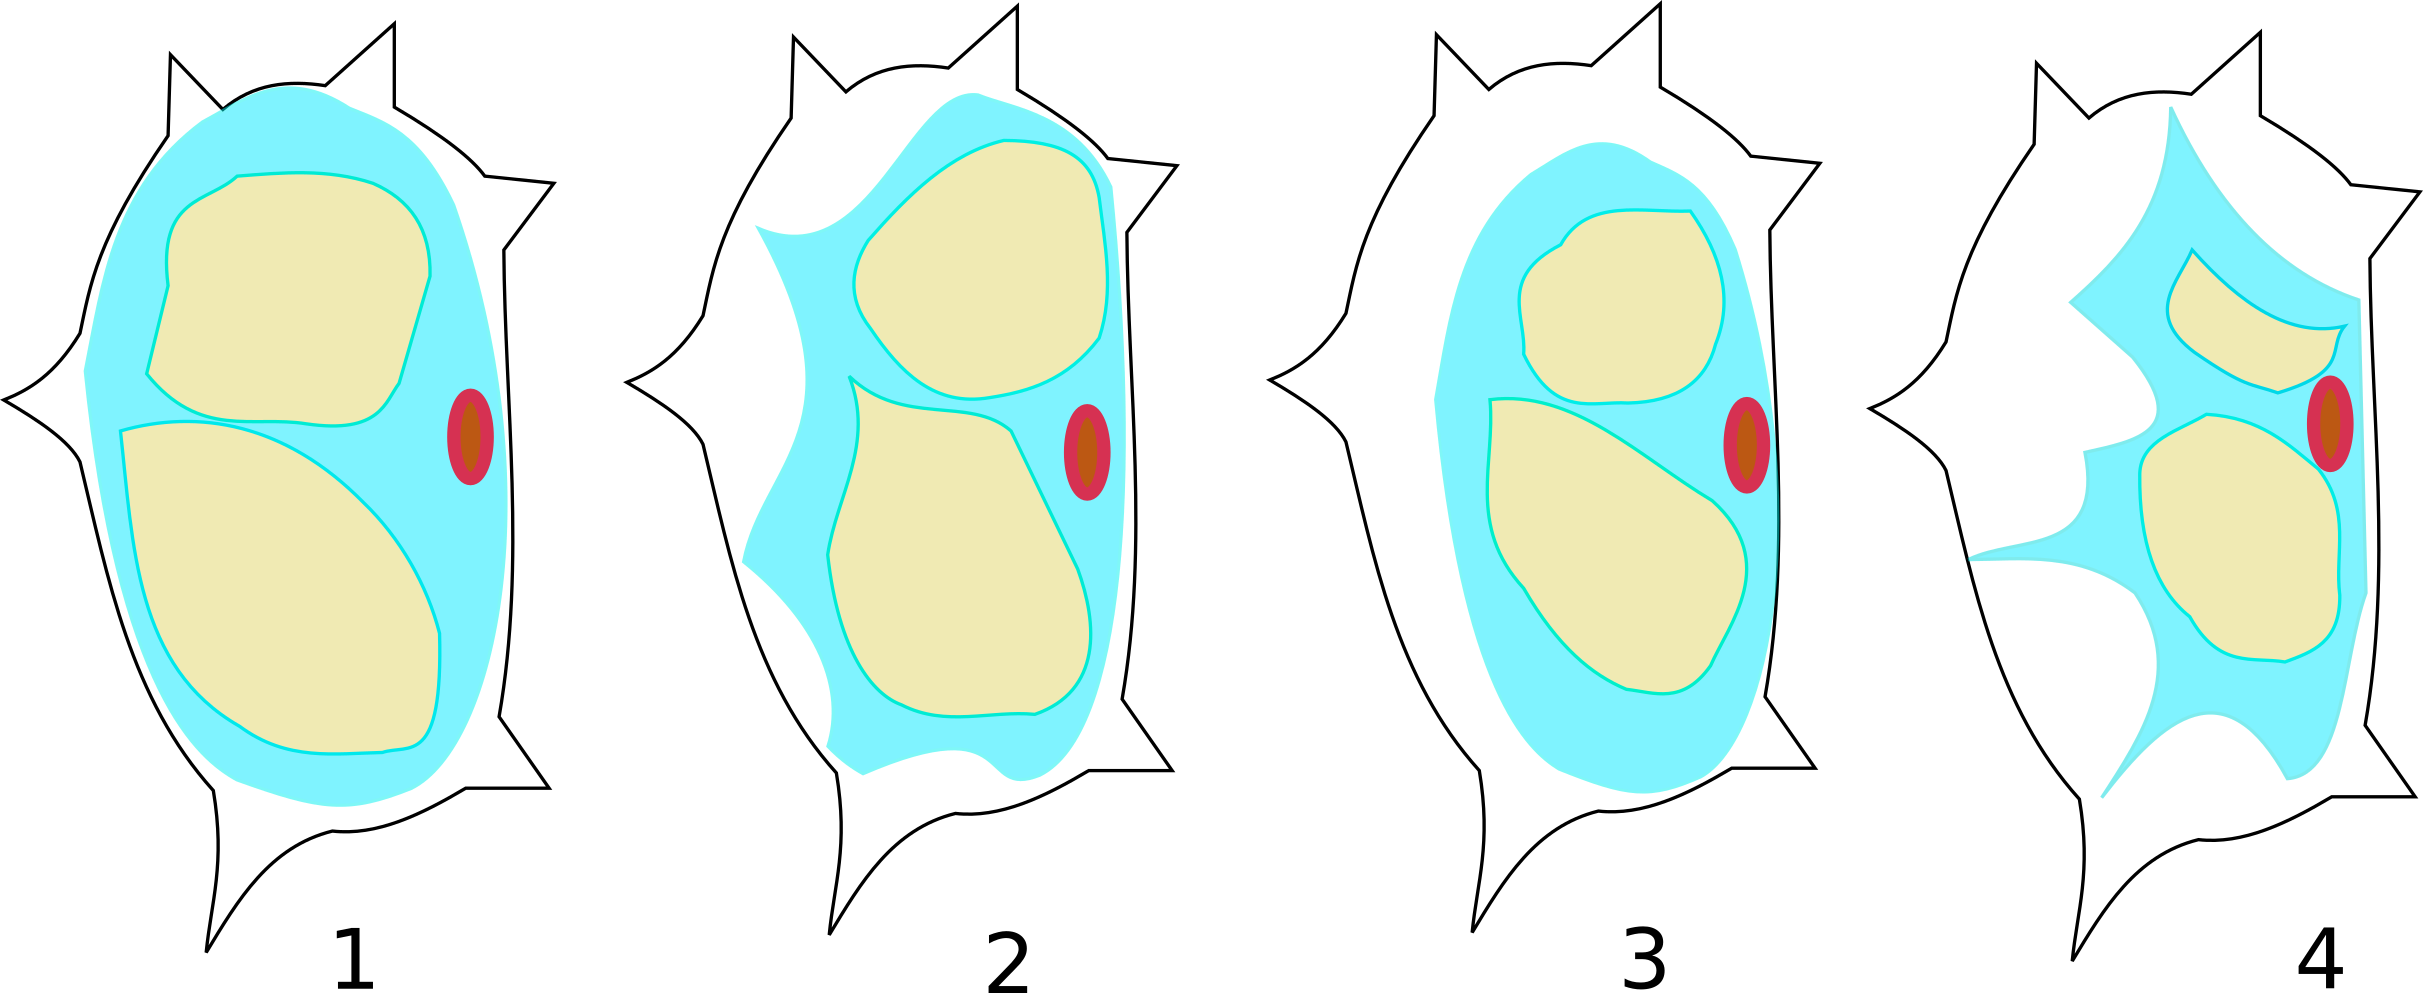
\includegraphics[width=0.5\linewidth]{pictures/plasmolis}
%\caption{Различные типы плазмолиза}
%\label{plasmolis_types}
%\end{figure}
%%%%%%%%%%%%%%%%%%%%%%%%%%%%%%%%%%%%%%%%%%%%%%%%%%%%%%%%%%%%%%%%%%%%%%%%%%%%%%%%%%%%%%%%%%%%%%%%%%%%%%%%%%%

%\paragraph*{}При определенных условиях, плазмолиз может быть \hyperlink{reversable_plasmolisys}{обратимым}. Явление обратное плазмолизу носит название \textit{деплазмолиз}.
%\paragraph{}Катионы и анионы солей оказывают специфическое и многообразное действие на цитоплазму. Одним из заметных внешних проявлений этого действия является изменение степени набухания и вязкости цитоплазмы. Чем выше вязкость цитоплазмы, тем медленнее наступает плазмолиз. Показателем, характеризующим особенности ответной реакции цитоплазмы на воздействие отдельных солей, служит время плазмолиза.

%\paragraph{}Одной из характеристик плазмолиза является время, необходимое для его начала. 

%\paragraph{}\efbox[margin=10pt,backgroundcolor=yellow]{
%	\begin{minipage}{0.95\textwidth}
%\textbf{Время плазмолиза} – это время, прошедшее от момента погружения ткани в гипертонический раствор соли, до наступления выпуклого плазмолиза (примерно у половины клеток в поле зрения микроскопа).
%	\end{minipage}
%	}

%\paragraph*{}Время наступления плазмолиза может зависеть от вязкости цитоплазмы. Чем выше вязкость цитоплазмы, тем медленнее наступает плазмолиз. В свою очередь на вязкость и степень набухания цитоплазмы оказывают влияние различные катионы, в первую очередь ионы K$^+$ и Ca$^{2+}$.


%\paragraph*{}При действии на клетку \hyperlink{hypertonik_liquid}{гипертонических} растворов солей, проникающих через плазмолемму, но не проходящих через тонопласт возникает \textit{колпачковый плазмолиз}, который проявляется  в образовании колпачков из набухшей цитоплазмы на концах плазмолизированного тонопласта.

%\paragraph*{}Соли, вызывающие колпачковый плазмолиз вызывают, кроме того, набухание цитоплазмы, денатурацию белков и увеличение светорассеяния.

\begin{footnotesize}

\paragraph*{}\textbf{Цель работы}: изучить, реакцию клетки на нарушение баланса катионов. Провести наблюдения плазмолиза различного типа

\paragraph*{}\textbf{Оборудование}: Луковица с пигментированными чешуями. Микроскопы, предметные и покровные стекла, бритвы, секундомер;

\paragraph*{}\textbf{Реактивы}: растворы солей: 0,7 М Ca(NO${_3}$)$_2$, 1M KNO$_3$, 1M KCNS;

\end{footnotesize}


\subsection*{Ход работы}

\paragraph*{}С выпуклой поверхности пигментированной чешуи лука срежьте участок эпидермиса и поместите его на предметное стекло в каплю раствора нитрата кальция. 

\paragraph*{}Накройте, подготовленный таким образом препарат кожицы лука, покровным стеклом и рассмотрите его под микроскопом, следя за сменой форм плазмолиза. 

\paragraph*{}С помощью секундомера определите время начала плазмолиза клеток.

\paragraph*{}Определите время плазмолиза для клеток эпидермиса, помещённых в раствор нитрата калия.

\paragraph*{}На примере препарата, помещённого в растворе родонида калия (KCNS) пронаблюдайте за наступлением колпачкового плазмолиза. 

\paragraph*{}Зарисуйте в альбом клетки, находящиеся на разных стадиях плазмолиза.

\paragraph*{}\textbf{Сделайте выводы}, в которых обоснуйте, каким образом плазмолиз доказывает тот факт, что цитоплазматическая мембрана является полупроницаемой.

\subsection*{Вопросы для самоконтроля}

	\begin{itemize}
		\item Дайте определение понятию \hypertarget{gomiostatsis_question}{гомеостаз}.
		\item Что такое осмотическое давление, в каких единицах оно измеряется. Что такое \hypertarget{hypertonik_liquid}{гипертонический}, гипотонический и изотонический растворы \cite{chem_kuzmenko_eremin}?
		\item От каких факторов зависит величина осмотического давления?
		\item Что такое тургорное давление?
		\item Наблюдаются ли различия в характере плазмолиза вызванного разными солями? Чем это можно объяснить?
		\item В растворах каких веществ будет наблюдаться \hypertarget{reversable_plasmolisys}{обратимый плазмолиз}? Почему?
		\item Способны ли плазмолизироваться мертвые клетки? Почему?
		\item Какова физическая природа процессов диффузии и осмоса?
		\item Каким образом ионы и вода проходят через цитоплазматическую мембрану клетки. В чем различия между активным и пассивным транспортом?
	\end{itemize}


\section*{\lbtitle Определение потенциального осмотического давления клеточного сока путем плазмолиза}

\addcontentsline{toc}{section}{Определение потенциального осмотического давления клеточного сока путем плазмолиза}

%\subsection*{Теоретические положения}

%\paragraph*{}Клеточный сок является сложным раствором разнообразных органических и неорганических соединений. Как и всякий раствор, клеточный сок характеризуется потенциальным осмотическим давлением, которое зависит от его концентрации, т.е. от числа частиц растворенного вещества, находящихся в этом растворе.

%\paragraph{}\efbox[margin=10pt,backgroundcolor=yellow]{
%	\begin{minipage}{0.95\textwidth}
%\textbf{Потенциальное осмотическое давление} (ПОД) - это показатель, который характеризует максимальную способность клетки всасывать воду. 
%	\end{minipage}
%	}

%\paragraph*{}Очевидно, что чем большим осмотическим давлением обладает клетка, тем выше ее способность к поглощению воды. По этой причине значение ПОД может быть использовано для оценки возможности произрастания растения на почвах с различной водоудерживающей силой. Так, наибольшим осмотическим давлением характеризуются клетки \hyperlink{xserofites}{растений-ксерофитов}, которые вынуждены извлекать воду из очень сухих почв и удерживать ее в своих клетках. 

%\paragraph*{}Величина \hypertarget{p_osm_other_plants}{ПОД} постоянно колеблется и различается как у разных видов растений, так и у растений одного вида, в разные периоды их жизненного цикла.  Например, низкое осмотическое давление – около 0,1 МПа наблюдается у водных растений. Осмотическое давление, равное 20,0 МПа, обнаружено у галофита \textit{Atriplex confertifolia}. У большинства растений средней полосы осмотическое давление колеблется от 0,5 до 3 МПа \cite{fzr_jakushina}. Повышение осмотического давления клеточного сока во время засухи служит критерием степени обезвоженности клетки.

\begin{footnotesize}

\paragraph*{}\textbf{Цель работы}: экспериментально определить величину потенциального осмотического давления клетки;

\paragraph*{}\textbf{Оборудование}: Луковица с пигментированными чешуями, микроскоп, предметные и покровные стекла, бритвы, бюксы, градуированные пипетки;

\paragraph*{}\textbf{Реактивы}: растворы сахарозы 0,1 М и KNO$_3$, 0,1M;

\end{footnotesize}

\subsection*{Ход работы}

\subsubsection*{Наблюдение плазмолиза в растворах различной концентрации}

\paragraph*{}В бюксах необходимо приготовить по 10 мл растворов сахарозы и KNO$_3$ различной концентрации. Данные растворы готовятся путем разбавления дистиллированной водой исходного 1 М раствора сахарозы согласно таблице \ref{pot_osm_press_work}.

\begin{table}[!h]

\label{pot_osm_press_work}
\caption{Рабочая таблица для расчета потенциального осмотического давления}
\begin{tabular}{|p{2cm}|p{2cm}|p{1.5cm}|p{1.5cm}|p{1.5cm}|p{1.5cm}|p{1.5cm}|p{1.5cm}|}


\hline Концентра\-ция раствора, \- моль/л & 1 моль раствора сахарозы, мл & воды мл & время погружения & время наблюдения & степень плазмолиза & изотони\-ческая концентра\-ция,\- моль/л & осмоти\-ческое давление, кПа \\
%\hline \rotatebox{90}{Концентрация раствора, \- моль/л} & 1 моль раствора сахарозы, мл & воды мл & время погружения & время наблюдения & \rotatebox{90}{степень плазмолиза} & \rotatebox{90}{изотоническая концентрация,\- моль/л} & \rotatebox{90}{осмотическое давление, кПа} \\
\hline 0,7 & 7 & 3 &  &  &  & &  \\
\hline 0,6 & 6 & 4 &  &  &  & &  \\
\hline 0,5 & 5 & 5 &  &  &  & &  \\
\hline 0,4 & 4 & 6 &  &  &  & &  \\
\hline 0,3 & 3 & 7 &  &  &  & &  \\
\hline 0,2 & 2 & 8 &  &  &  & &  \\
\hline 0,1 & 1 & 9 &  &  &  & &  \\
\hline

\end{tabular}

\end{table}

\paragraph*{}Сделайте тонкий срез эпидермиса с выпуклой стороны пигментированной чешуи луковицы.

\paragraph*{}Затем, с интервалом времени в 3 минуты, поместите полученные срезы чешуй (по 2-3) в каждый из бюксов с приготовленными растворами, начиная с того бюкса, в котором концентрация раствора самая высокая (0,7 М). 
Через 30 минут извлеките срезы из первого бюкса и исследуйте их под микроскопом. Срезы из остальных бюксов извлекаются, через каждые 3 минуты и так же исследуются под микроскопом. 

\paragraph*{\warningsign}Срезы исследуются в капле того раствора, из которого их извлекли.

\paragraph*{}В каждом из исследуемых под микроскопом срезов определите степень выраженности плазмолиза. На основе этих наблюдений – \textit{\hypertarget{c_isitonik}{изотоническую концентрацию}} клеточного сока, которая рассчитывается как среднее арифметическое между концентрацией раствора, в котором ещё не наблюдается плазмолиза и концентрации раствора, в котором плазмолиз уже начался.

\paragraph*{}Результаты опыта запишите в таблицу \ref{pot_osm_press_work}.

\paragraph*{}Потенциальное осмотическое давление цитоплазмы клетки рассчитывается по формуле \ref{p_osmotick_formula}:

\begin{equation}
\label{p_osmotick_formula}
	P = RTci
\end{equation}

\paragraph*{}Где \textit{P} - потенциальное осмотическое давление, \textit{R} - универсальная газовая постоянная Больцмана, равная 8,3 Дж/Моль*К, c - изотоническая концентрация, найденная \hyperlink{c_isitonik}{ранее} опытным путем, i - изотонический коэффициент Вант-Гоффа, который показывает степень ионизации раствора и определяется по формуле \ref{i_isotonik}:

\begin{equation}
	\label{i_isotonik}
	i = 1 + \alpha(n + 1)
\end{equation}

\paragraph*{}Где $\alpha$ - степень диссоциации раствора данной концентрации, n - число ионов, на которое диссоциирует данное вещество. Например, для KNO$_3$ n = 2, так как данная соль диссоциирует с образованием двух ионов:

\begin{equation}
	KNO_3 \rightarrow K{^+} + NO{_3}{^-}
\end{equation}

\paragraph*{}Для сахарозы, которая не является электролитом и не диссоциирует, n = 1.

\paragraph*{}Ниже приводится степень диссоциации KNO$_3$ в зависимости от концентрации раствора

\begin{table}[h!]
\centering
\caption{Степень диссоциации KNO$_3$ в зависимости от концентрации раствора}
	\begin{tabular}{|c|c|c|c|c|c|}
	
	\hline Концентрация. M     & 0,5  & 0,4  & 0,3  & 0,2  & 0,1 \\
	\hline Степень диссоциации & 0,71 & 0,74 & 0,76 & 0,79 & 0,83 \\
	\hline
	\end{tabular}
	
\paragraph*{}Таблица приведена согласно \cite{vorob_2013}
\end{table}

\paragraph*{}\textbf{Сделайте вывод}, в котором сопоставьте определенную вами в опыте величину осмотического давления клеток кожицы лука с величиной осмотического давления клеток других \hyperlink{p_osm_other_plants}{растений} , которые упоминаются в теоретических положениях к данному опыту.

\subsection*{Вопросы для самоконтроля}

	\begin{itemize}
		\item Какие растения относятся к \hypertarget{xserofites}{ксерофитам}? Какими чертами организации они обладают?
		\item Что такое коллигативные свойства раствора. Перечислите эти свойства;
		\item Почему во время засухи осмотическое давление в клетках растения повышается?
		\item Что такое водный потенциал клетки, каковы его составляющие?
		\item Какое практическое значение имеет определение величины осмотического давления клеток растения?
 	
	\end{itemize}

%\chapter{Водный обмен растения}

%\paragraph*{}Все физиологические процессы в организме растения, могут нормально протекать только при условии полной обеспеченности растения \hypertarget{whater_balance}{водой}. Ток воды по сосудам проводящих тканей – \hyperlink{xsilema_tisue}{ксилемы и флоэмы} обеспечивает в организме растения транспорт веществ и, таким образом, связывает в единую систему различные органы растений. Тургорное давление внутри клеток, вызванное давление цитоплазмы на клеточную стенку, обеспечивает прочность растительных тканей. 

%\paragraph*{}Движение воды по растению происходит из области с высоким водным потенциалом (почва), в область с низким (атмосфера).

%\paragraph*{}Водный обмен растений складывается из трех этапов:

%\begin{itemize}
%	\item Поглощение воды
%	\item Транспорт воды 
%	\item Испарение воды
%\end{itemize}

%\paragraph*{}Поглощение растением воды происходит через корневые волоски –  выросты клеток эпидермиса корня в зоне поглощения. Через корневые волоски вода поступает в корень вследствие разности осмотического давления почвенного раствора и клеточного сока клеток корня. Для увеличения осмотического давления в корне, растение накапливает в его клетках ионы K$^+$ \cite{fzr_ermakov}. Механизм поступления воды через корень носит название нижний концевой двигатель. 

%\paragraph*{}Доказательством действия присасывающей силы корня служит <<плач растений>>, когда на свежесрезанном стебле образуются капли воды, которая нагнетается в стебель корневым давлением.

%\paragraph*{}Транспорт воды из корня в листья осуществляется по сосудам ксилемы. Сосуды этой ткани образованы мёртвыми клетками с узким просветом. Удержание водной нити в сосуде происходит за счёт сцепления молекул воды с их стенками – \textbf{адгезии}. Кроме того, молекулы воды удерживаются вмести за счёт межмолекулярных взаимодействий молекул воды - \textbf{когезии}. Адгезия и когезия препятствуют образованию в просвете сосуда полостей заполненных воздухом. 

%\paragraph*{}Испарение воды листьями приводит к снижению водного потенциала в их мезофилле. Таким образом, разность водного потенциала обеспечивает движение воды от корня к листьям.

%\paragraph*{}Испарение воды происходит главным образом через устьица (рисунок \ref{ustitsa}). Данный процесс носит название \textit{\hyperlink{transpiration_question}{транспирация}}. В результате потери воды клетками в них снижается водный потенциал и возрастает сосущая сила. Это приводит к усилению поглощения воды клетками листа из ксилемы жилок и поступлению воды из корня в листья. Этот механизм поступления воды называется \textbf{верхним концевым двигателем}. 

%%%%%%%%%%%%%%%%%%%%%%%%%%%%%%%%%%%%%%%%%%%%%%%%%%%%%%%%%%%%%%%%%%%%%%%%%%%%%%%%%%%%%%%%%%%%%%%%%%%%%%%%%%% 
%\begin{figure}
%  \centering
%       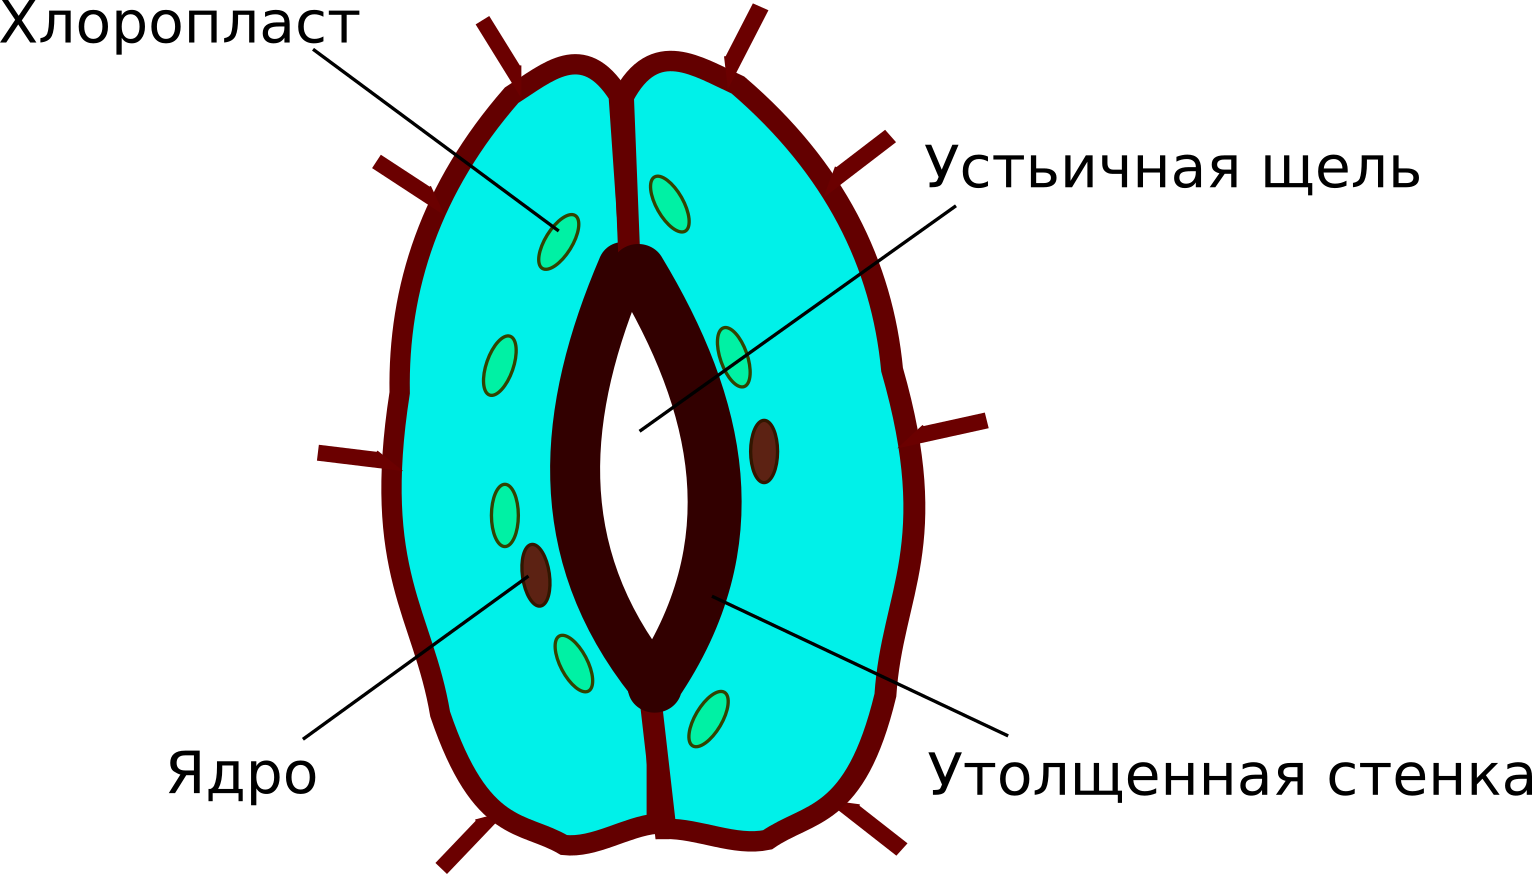
\includegraphics[width=0.5\linewidth]{pictures/ustitsa}
%\caption{Строение устьица}
%\label{ustitsa}
%\end{figure}
%%%%%%%%%%%%%%%%%%%%%%%%%%%%%%%%%%%%%%%%%%%%%%%%%%%%%%%%%%%%%%%%%%%%%%%%%%%%%%%%%%%%%%%%%%%%%%%%%%%%%%%%%%%%

\section*{\lbtitle Определение интенсивности транспирации весовым методом}
\addcontentsline{toc}{section}{Определение интенсивности транспирации весовым методом}

%\subsection*{Теоретические положения}

%\paragraph{}\efbox[margin=10pt,backgroundcolor=yellow]{
%	\begin{minipage}{0.95\textwidth}
%	Интенсивность транспирации — это величина, показывающая количество воды испаряющейся с единицы поверхности листа за единицу времени. 
%	\end{minipage}
%	}
	
%\paragraph{}\hyperlink{transpiration_intensivity}{Данная величина} зависит от ряда внешних факторов, таких, как \hyperlink{transpiration_time}{времени суток}, температура, \hyperlink{transpiration_air_humidity}{относительная влажность воздуха} и обычно колеблется в пределах 15-250 г/(м$^2$*ч).

%\paragraph*{}Для определения интенсивности транспирации чаще всего используется весовой метод, который основан на учете потери растением воды при испарении. Весовым методом можно изучать как транспирацию целого растения, так и отдельных его частей. Так как определить интенсивности транспирации у целого растения довольно сложно, чаще всего измерения проводят на срезанных побегах и листьях. Чтобы во время опыта оводненность тканей не снижалась, срезанный лист помещают в прибор Веска, заполненный водой (рисунок \ref{veska}).

%\paragraph*{}Транспирация это физиологически активный процесс и растения способны в некоторых пределах регулировать его интенсивность. Способность растений к регуляции интенсивности транспирации характеризует такой показатель как \textit{относительная транспирация}. 

%\paragraph{}\efbox[margin=10pt,backgroundcolor=yellow]{
%	\begin{minipage}{0.95\textwidth}
%	Относительная транспирация — это отношение интенсивности транспирации к интенсивности испарения со свободной водной поверхности при тех же условиях. 
%	\end{minipage}
%	}	
	
%\paragraph{}Относительная транспирация обычно составляет 0,1-0,5.

\begin{footnotesize}

\paragraph*{}\textbf{Цель работы}: Определить весовым методом интенсивность транспирации у подсолнечника;

\paragraph*{}\textbf{Оборудование}: Трехнедельные растения подсолнечника, аналитические весы, часы, прибор Веска, чашки Петри, ножницы, бумага, линейка, вата;

\end{footnotesize}

\subsection*{Ход работы}

\subsubsection*{Подготовка прибора Веска}

\paragraph*{}Со стебля используемого для опыта растения, срежьте лист вместе с черешком. Черешок срезанного листа поместите в отверстие резиновой пробки прибора Веска и  плотно укрепите там ватой. 

\paragraph*{\warningsign}Следует помнить, что конец черешка должен выступать из нижней части пробки настолько, чтобы в собранном приборе он был погружен в воду. 

\paragraph*{}Нижний конец черешка подрезается наискось под водой примерно на 1 см. Эта операция необходима для восстановления водяных нитей в проводящих сосудах. Пробка с укрепленным на ней листом вставляется в прибор Веска, наполненный водой комнатной температуры (рисунок \ref{veska}).  

%%%%%%%%%%%%%%%%%%%%%%%%%%%%%%%%%%%%%%%%%%%%%%%%%%%%%%%%%%%%%%%%%%%%%%%%%%%%%%%%%%%%%%%%%%%%%%%%%%%%%%%%%%% 
\begin{figure}[h]
  \centering
       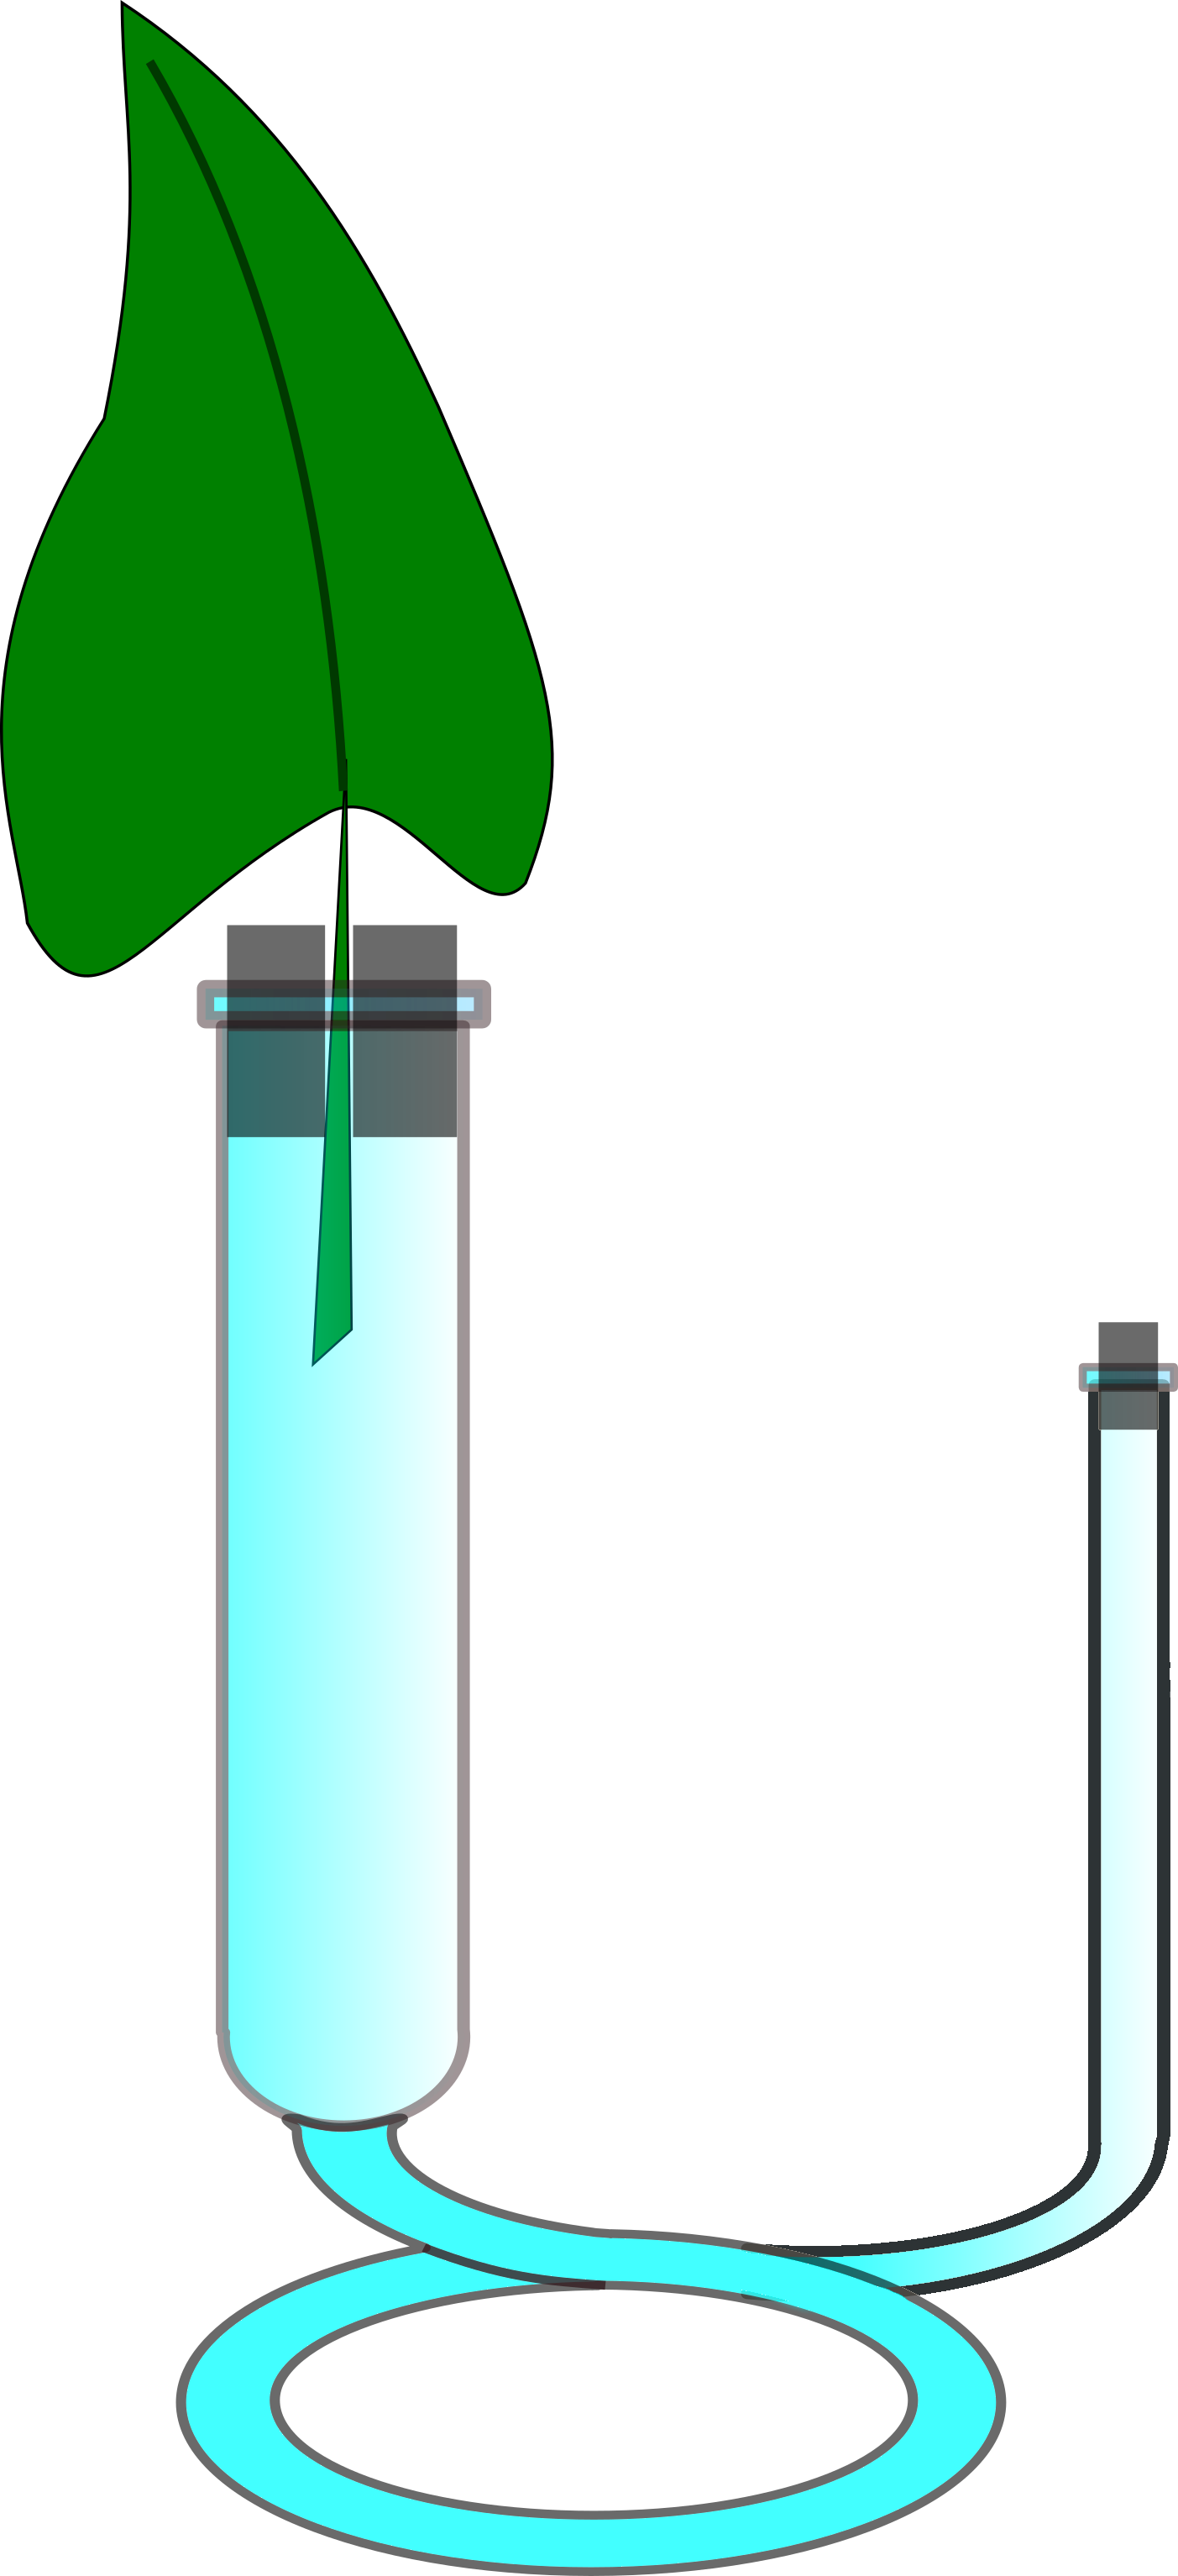
\includegraphics[width=0.2\linewidth]{pictures/veska}
\caption{Прибор Веска в собранном виде}
\label{veska}
\end{figure}
%%%%%%%%%%%%%%%%%%%%%%%%%%%%%%%%%%%%%%%%%%%%%%%%%%%%%%%%%%%%%%%%%%%%%%%%%%%%%%%%%%%%%%%%%%%%%%%%%%%%%%%%%%%

\paragraph*{}Для обеспечения точности измерения, смонтированный и готовый к работе прибор Веска должен быть совершенно сухим, плотно закрытым, пробка не должна касаться воды.

\paragraph*{}Описанным выше образом необходимо приготовить два прибора Веска. Перед началом опыта, приборы с закрепленными листьями необходимо взвесить на аналитических весах и снабдить этикетками с указанием веса прибора. Один из приборов помещается под прямой солнечный свет, например на окно лаборатории, а другой в \hyperlink{light_dark_diferences}{темную камеру}. 

\paragraph*{}Через 1 час после начала опыта взвести приборы повторно. По разнице с первоначальной массой установите количество воды, которое испарил лист за время опыта.

\subsubsection*{Измерение площади листа}

\paragraph*{}Для того, чтобы выполнить расчеты интенсивности транспирации, необходимо знать площадь листа. Площадь листа измеряется следующим способом: из бумаги вырезается квадрат со стороной 10 см. Таким образом, площадь этого квадрата будет составлять 100 см$^2$. Приготовленный для опыта лист необходимо приложить к бумаге, обвести карандашом и вырезать по полученному контуру. 

\paragraph*{}Затем на аналитических весах определите массу квадрата и бумажного контура листа. Площадь листа определяется по пропорции \ref{liaf_square}: 

\begin{equation}
  \label{liaf_square}
  S_l = \frac{S_{sq} * m_k}
                 {m_{sq}}
\end{equation}

\paragraph*{}Где $S_{l}$ – площадь листа, $S_{sq}$ – площадь бумажного квадрата, $m_k$ – масса квадрата, $m_{sq}$ – масса квадрата.

\subsubsection*{Вычисление интенсивности транспирации}

\paragraph*{}На основании полученных результатов рассчитайте интенсивность транспирации, то есть количество воды в граммах, которое испаряет единица листовой поверхности (1м$^2$) в единицу времени (1 ч).

\paragraph*{}Интенсивность транспирации рассчитывается  по следующей формуле \ref{transpiration_level} 

\begin{equation}
	\label{transpiration_level}
	T = \frac{10000*C}{St}
\end{equation}

\paragraph*{}Где \textit{T} - интенсивность транспирации, \textit{C} - убыль массы листа за время опыта; \textit{S} - площадь листа (м$^2$); \textit{t} - время опыта (ч)

\paragraph*{}\textbf{Сделайте вывод} о там, как сильно отличается уровень транспирации у растения в темноте и на свету. На основе знания о механизме работы устьиц \cite{fzr_ermakov, fzr_jakushina} обоснуйте почему.

\subsection*{Вопросы для самоконтроля}

	\begin{itemize}
		\item Опишите строение клеток \hypertarget{xsilema_tisue}{ксилемы и флоэмы}. Благодаря каким особенностям строения клетки этих тканей приспособлены к транспорту воды?
		\item Из каких компонентов складывается водный режим растения?
		\item Что такое \hypertarget{transpiration_question}{транспирация}? В чем заключается значение транспирации для растения?
		\item От каких факторов зависит \hypertarget{transpiration_intensivity}{интенсивность транспирации}?
		\item \hypertarget{transpiration_air_humidity}{Почему} интенсивность транспирации снижается при повышении относительной влажности воздуха?
		\item Почему сильный ветер способствует более интенсивной транспирации?
		\item \hypertarget{transpiration_time}{В какое время суток} интенсивность транспирации наибольшая. Почему?
		\item Опишите механизм работы устьиц;
		\item Каким образом растения-ксерофиты уменьшают потерю влаги через устьица?
		\item \hypertarget{light_dark_diferences}{Есть} ли различия в интенсивности транспирации побегов на свету и в темноте? Как можно объяснить результаты опыта?
		\item Что такое вещества-антитранспиранты? какие группы антитранспирантов вы знаете;
	\end{itemize}

\section*{\lbtitle Наблюдение за движением устьичных клеток под микроскопом} 

%\subsection*{Теоретические положения}

%\paragraph*{}Через устьица приходит испарение воды и газообмен между растением и атмосферой. Каждое устьице состоит из замыкательных клеток бобовидной (у двудольных) или гантелевидной (у однодольных) растений формы. Работа устьиц обеспечивается неравномерным утолщением их клеточных стенок, за счет чего, замыкающие клетки устьиц в состоянии тургора выгибаются, открывая, таким образом, устьичную щель. За счет работы устьиц растение может активно регулировать уровень испарения воды с поверхности своих листьев.

\begin{footnotesize}

\paragraph*{}\textbf{Цель работы}: Наблюдение за работой устьичного аппарата под микроскопом;

\paragraph*{}\textbf{Оборудование}: Листья традесканции, лезвия, препаровальные иглы, предметные и покровные стекла, фильтровальная бумага, микроскоп;

\paragraph*{}\textbf{Реактивы}: Раствор сахарозы 1 М; Раствор глицерина 5\%, вода;

\end{footnotesize}

\subsection*{Ход работы}

\subsubsection*{Наблюдение работы устьичного аппарата в растворе сахарозы}

\paragraph*{}На предметное стекло, в каплю воды, поместите срез эпидермиса нижней стороны листа. Рассмотрите под микроскопом устьица, зарисуйте в рабочей тетради строение устьица и отметить на рисунке утолщения внутренней стенки замыкательных клеток устьиц. 

\paragraph*{}Затем, с помощью фильтровальной бумаги замените воду на предметном стекле на раствор сахарозы и наблюдайте за изменениями устьица. В рабочей тетради нужно зарисовать устьице в закрытом состоянии. Снова замените воду на предметном стекле на раствор сахарозы и наблюдайте за закрытием устьица.

\subsubsection*{Наблюдение работы устьичного аппарата в растворе глицерина}

\paragraph*{}Поместить срез эпидермиса листа в раствор глицерина и наблюдать плазмолиз в замыкательных клетках устьиц. В следствии плазмолиза устьичные клетки закрываются, но через некоторое время открываются вновь. Это происходит из за того, что глицерин проникает в цитоплазму устьичных клеток, вызывая их деплазмолиз.

\paragraph*{}Замените глицерин на предметном стекле на воду. Для этого с одной стороны капните на предметное стекло каплю воды, а с другой оттяните глицерин с помощью фильтровальной бумаги. Устьица откроются еще шире, чем это было в начале опыта, так как после проникновения в цитоплазму замыкательных клеток глицерина, осмотическое давление в этих клетках начинает повышаться.

\paragraph*{}Результаты наблюдений запишите в тетрадь.

\paragraph*{}\textbf{Сделайте вывод} как проведенные вами наблюдения согласуются с известными вами сведениями о механизме работы устьиц.

\subsection*{Вопросы для самоконтроля}

\begin{itemize}
	\item Какое приспособительное значение имеет расположение устьиц на нижней стороне листа?
	\item Какое значение для работы устьица имеет неравномерное утолщение стенки замыкательной клетки устьица?
	\item В какое время суток устьица в растении находятся в раскрытом состоянии. Почему?
	\item Почему осмотическое давление клеточного сока замыкательных клеток устьиц повышается на свету?
\end{itemize}

	
%\chapter{Фотосинтез}

%\paragraph{}\efbox[margin=10pt,backgroundcolor=yellow]{
%	\begin{minipage}{0.95\textwidth}
%	\hypertarget{fotosintethis}{Фотосинтез} - это процесс синтеза органических веществ из неорганических за счет энергии солнечного света и при участии пигмента хлорофилла. 
%	\end{minipage}
%	}	
	
%\paragraph{}Первичными продуктами фотосинтеза являются моносахариды, в частности глюкоза, запас которой сохраняется в растении в виде крахмала.

%\paragraph*{}Реакции фотосинтеза протекают в специализированных органеллах – хлоропластах в две стадии. В ходе световой стадии за счёт энергии квантов света из атома магния, входящего в состав  хлорофилла, выбиваются электроны, которые за счёт работы ферментов электрон-транспортной цепи перемещаются на внешнюю част мембраны хлоропласта. Одновременно с этим протоны, которые образуются в результате фотолиза воды, накапливаются на внутренней части мембраны. Кислород, который выделяют растения, является при этом побочным продуктом фотолиза воды. 

%\paragraph*{}За счёт перераспределения протонов и электронов, на мембране возникает разность потенциалов. Когда разность потенциалов достигает определённого значения, протоны начинают двигаться к электронам через канал образованный ферментом АТФ-синтетазой. Энергия, выделяющаяся при этом, используется для синтеза АТФ, а протоны и электроны связываются со специальными белками-переносчиками - НАДФ.

%\paragraph*{}На темновой стадии, в ходе реакций цикла Кальвина, протоны, электроны и CO$_{2}$ используются для синтеза углеводов.

\section*{\lbtitle Определение химических свойств пигментов листа}
\addcontentsline{toc}{section}{Определение химических свойств пигментов листа}

%\subsection*{Теоретические положения}

%\paragraph*{}Хлоропласты высших растений содержат в себе два типа пигментов - хлорофилл \textit{a} и \textit{b} и каротиноиды. Хлорофилл принимает в процессе фотосинтеза активное участие: под действием энергии солнечного света он передает свой электрон в элеткрон-транспортную цепь. Остальные пигменты передают энергию лишь на хлорофилл \textit{а}. 

%\paragraph*{}По химической природе \hypertarget{chlorophilus_eterus}{хлорофиллы} \textit{а} и \textit{b} – \hyperlink{hlorpophilus_etherus}{сложные эфиры} дикарбоновой кислоты хлорофиллина и двух спиртов – метанола и фитола. В центре молекулы хлорофилла расположен атом магния, соединенный с четырьмя атомами азота пиррольных колец (рисунок \ref{chlorophill}).

%\paragraph*{}Молекулу хлорофилла состоит из гидрофильного порфиринового ядра и гидрофобного хвоста из спирта фитола. 

%%%%%%%%%%%%%%%%%%%%%%%%%%%%%%%%%%%%%%%%%%%%%%%%%%%%%%%%%%%%%%%%%%%%%%%%%%%%%%%%%%%%%%%%%%%%%%%%%%%%%%%%%%% 
%\begin{figure}
%  \centering
%       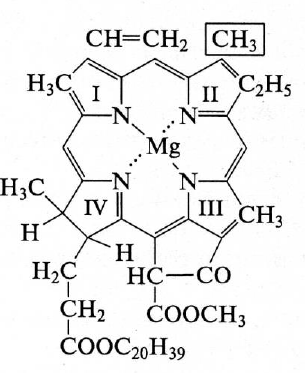
\includegraphics[width=0.3\linewidth]{pictures/chlorophill}
%\caption{Структура молекулы хлорофилла}
%\label{chlorophill}
%\end{figure}
%%%%%%%%%%%%%%%%%%%%%%%%%%%%%%%%%%%%%%%%%%%%%%%%%%%%%%%%%%%%%%%%%%%%%%%%%%%%%%%%%%%%%%%%%%%%%%%%%%%%%%%%%%%

%\paragraph*{}Фитол служит молекуле хлорофилла гидрофобным якорем, который удерживает гидрофильную порфириновую головку хлорофилла на мембране хлоропласта.

%\paragraph*{}Каротиноиды – по своей химической природе являются полиеновыми углеводородами состоящие из 40 атомов углерода и обладающие системой сопряженных двойных связей. Каротиноиды присутствуют в хлоропластах всех растений. В зеленых листьях присутствие каротиноидов скрывается хлорофиллом и они незаметны. Осенью хлорофилл в листьях разрушается, а каротиноиды остаются. За счет этого листья приобретают желтый и красный цвет.

\begin{footnotesize}

\paragraph*{}\textbf{Цель работы}: Изучить основные химические свойства пигметов листа

\paragraph*{}\textbf{Оборудование}: Сухие или свежие листья, конические колбы с обратным холодильником, водяная баня, штатив с пробирками, пипетки на 1 мл, конические колбочки, воронки, цветные карандаши.

\paragraph*{}\textbf{Реактивы}: Этиловый спирт, бензин, 20\%-й раствор NaOH, 10\%-й раствор соляной кислоты, ацетат меди.

\end{footnotesize}

\subsection*{Ход работы}

\subsubsection*{Получение спиртовой вытяжки хлорофилла}

\paragraph*{}Измельчите ножницами приготовленные для опыта свежие листья, а затем разотрите их в ступке вместе с частицами мела и песка, постепенно подливая в ступку этиловый спирт. 

\paragraph*{}Полученную массу необходимо слить из ступки в колбу через бумажный фильтр. Закройте колбу, содержащую этот раствор пробкой и поместите на водяную баню с кипящей водой на пять минут. Полученная таким образом спиртовая вытяжка хлорофилла будет использоваться в последующих опытах.

\subsubsection*{Разделение пигментов по Краусу}

\paragraph*{}Данный метод основан на различной растворимости пигментов в спирте и бензине. Пигменты разделяются благодаря тому, что спирт и бензин не смешиваются, и находясь в одном сосуде образуют две фазы – верхнюю бензиновую и нижнюю спиртовую.

\paragraph*{}Налейте в пробирку 2-3 мл спиртовой вытяжки пигментов, приготовленной на предыдущем этапе, и добавьте к данной вытяжке 3-4 мл бензин. Затем плотно закройте пробирку пробкой и несколько раз энергично встряхните, для того чтобы жидкости, находящиеся в пробирке смешались. После этого дайте пробирке отстояться.

\paragraph*{}В результате разной растворимости пигментов, хлорофилл и каротиноиды переходят бензин, и бензин окрашивается в зелёный цвет. Ксантофилл остаётся в спиртовом слое и придаёт ему золотисто-жёлтую окраску. 

\paragraph*{}Если пигменты разделяются недостаточно чётко, добавьте в пробирку три-четыре капли воды и снова встряхните. 

\paragraph*{}Зарисуйте в отчет окраску слоёв, укажите на рисунке распределение пигментов (рисунок \ref{pigments_separation}).

\begin{figure}[h!]
\label{pigments_separation}
\caption{Схема распределения пигментов в пробирке}
	\begin{tikzpicture}
		
		\draw[rounded corners=1pt] (-0.1,4) rectangle (2.1,4.1);
		\draw (0,0) rectangle (2,4);
		\draw (0,0) rectangle (2,1);
		\draw (2,0) arc [start angle=0, end angle=-180, radius=1];
		\path[draw=red](1.5,0.5) -- (3,1);
		\path (3,1)--(5,1) node{Цвет? Пигменты?};
		\path[draw=red](1.5,-0.5) -- (3,-1);
		\path (3,-1)--(5,-1) node{Цвет? Пигменты?};

		
	\end{tikzpicture}
\end{figure}

\subsubsection*{Омыление хлорофилла щелочью}

\paragraph*{}Как было сказано \hyperlink{chlorophilus_eterus}{выше}, по своей химической природе хлорофилл является сложным эфиром. По этой причине,  при обработке хлорофилла щелочью, можно вызвать омыление эфирных групп, то есть отщепление остатков метилового спирта и фитола.

\chemfig{C_{32}H_{30}ON_{4}Mg(-[1]COOCH_{3})(-[7]COOC_{20}H_{39})} + 2NaOH $\rightarrow$ \chemfig{C_{32}H_{30}ON_{4}Mg(-[1]COONa)(-[7]COONa)} +  CH$_{3}$OH + C$_{20}$H$_{39}$OH


\paragraph*{}В результате омыление образуется соль хлорофилловой кислоты, которая сохраняет зеленую окраску хлорофилла, но при этом приобретает гигрофильные свойства в следствии  отсутствия фитольного хвоста.  

\paragraph*{}Для проведения опыта в пробирку с 2-3 мл ранее полученной вытяжки хлорофилла прилейте 1 мл 20\%-го раствора NaOH.

\paragraph*{}Взболтайте полученную смесь и на несколько минут поместите ее на водяную баню.

\paragraph*{}После вскипания смеси, снимите пробирку с водяной бани и охладите, опустив низ пробирки в ёмкость с холодной водой. К охлаждённому раствору прилейте равный объем бензина и резко встряхните пробирку. В результате каротин и ксантофилл переходят в бензиновый слой, а натриевая соль хлорофилловой кислоты остаётся в спиртовом растворе.

\paragraph*{}Зарисуйте окраску слоёв в отчет и укажите распределение пигментов.

\subsubsection*{Получение феофитина и обратное замещение водорода атомом металла}

\paragraph*{}Атом магния сравнительно слабо удерживается внутри порфиринового кольца и, при условии мягкого воздействия, под действием кислоты может замещаться на два атома водорода. При этом образуется вещество бурого цвета - феофитин. 

\chemfig{C_{32}H_{30}ON_{4}Mg(-[1]COOCH_{3})(-[7]COOC_{20}H_{39})} + 2HCl $\rightarrow$ \chemfig{C_{32}H_{32}ON_{4}(-[1]COOCH_{3})(-[7]COOC_{20}H_{39})} +  MgCl$_{2}$

\paragraph*{}Если на феофитин подействовать солями металлов, например меди, то ион металла встроится в порфириновое кольца, а раствор хлорофилла вновь приобретет зеленую окраску. Это доказывает, что зеленый цвет растений обусловлен присутствием в составе хлорофилла магния.

 \chemfig{C_{32}H_{32}ON_{4}(-[1]COOCH_{3})(-[7]COOC_{20}H_{39})} + Cu(CH$_{3}$COO)$_{2}$ $\rightarrow$ \chemfig{C_{32}H_{30}ON_{4}Cu(-[1]COOCH_{3})(-[7]COOC_{20}H_{39})} +  2CH$_{3}$COOH

\paragraph*{}Для проведения опыта в две пробирки налейте по 2-3 мл спиртовой вытяжки пигментов и добавьте по две капли 10\%-го раствора соляной кислоты. При взбалтывании зелёная окраска хлорофилла переходит в бурую, характерную для феофитина. 

\paragraph*{}Оставьте одну пробирку с феофитином в качестве контроля, а во вторую поместите несколько кристаллов ацетата меди. Обе пробирки поместите на водяную баню и нагрейте до кипения. При нагревании бурый цвет раствора меняется на зелёный в результате образования хлорофиллоподобного производного меди.

\paragraph*{}Зарисуйте в отчет окраску феофитина и медьпроизводного хлорофилла.

\paragraph*{}\hypertarget{hlorpophilus_etherus}{На} основе проведенных опытов \textbf{сделайте вывод} о химической природе хлорофилла.

\subsection*{Вопросы для самоконтроля}

\begin{itemize}
 \item Какие еще группы фотосинтетических организмов вы знаете?
 \item В чем суть симбиотической теории возникновения хлоропластов?
 \item Что такое светособирающий комплекс и фотосистема?
 \item Что такое фотосинтетически-активная радиация?
 \item Что такое компенсационная точка фотосинтеза? Что произойдет с растением, находящимся в условиях освещенности ниже компенсационной точки?
 \item В чем состоит суть \textit{C-4} пути фотосинтеза. Фотосинтез каких растений идет по данному пути?
\end{itemize}

%\chapter{Дыхание}

%\paragraph{}\efbox[margin=10pt,backgroundcolor=yellow]{
%	\begin{minipage}{0.95 \textwidth}
%		\textbf{\hypertarget{breazting}{Дыхание}} - это процесс в результате которого окисление органических веществ ведет к выделению энергии. Выделенная энергия связывается в виде макроэргических связей в молекуле АТФ. 
%	\end{minipage}
%	}

%\paragraph*{}Основными веществами, которые расщепляются в ходе дыхания (субстратом дыхания) являются углеводы, в частности глюкоза. В том случае, если резерв углеводов иссякает, организм начинает расщеплять липиды а затем белки.

%\paragraph*{}По типу своего дыхания, большинство организмов являются аэробами, то есть процесс дыхания этих организмов идёт с поглощением кислорода. В процессе дыхания в результате передачи электронов по системе взаимосвязанных молекул белков - электрон-транспортной цепи (ЭТЦ) высвобождается энергия, заключённая в химических связях органического вещества. При этом кислород служит конечным акцептором электронов, прошедших через ЭТЦ. Дыхание является окислительно-восстановительным процессом, так как при потере электрона молекула окисляется, а при его присоединении - восстанавливается.

%\paragraph*{}Клеточное дыхание идет в две стадии. Первая из них - анаэробная стадия или гликолиз протекает в цитоплазме клетки. В ходе гликолиза молекула глюкозы расщепляется на две молекулы пировиноградной кислоты (ПВК) и синтезируются две молекулы АТФ.

%\paragraph*{}Второй этап аэробного дыхания проходит в специализированных органеллах - митохондриях. В цитоплазме митохондрии пировиноградная кислота в результате реакций цикла Кребса окисляется до CO$_{2}$. В процессе окисления от ПВК последовательно отщепляются и связываются со специальным ферментом-переносчиком протоны  и электроны. В дальнейшем, за счет работы электрон-транспортной цепи, на мембране митохондрии создается разность потенциалов, так как протоны оказываются на внешней стороне мембраны митохондрии, а электроны на внутренней. Когда разность потенциалов достигает определенного значения, протоны начинают двигаться к электронам через канал образованный ферментом АТФ-синтетазой. Энергия, выделяющаяся при этом, идет на синтез АТФ, а <<отработанные>>  протоны и электроны связываются с кислородом, образуя воду H$_{2}$O.

\section*{\lbtitle Определение интенсивности дыхания семян в закрытом сосуде}
\addcontentsline{toc}{section}{Определение интенсивности дыхания семян в закрытом сосуде}


%\subsection*{Теоретические положения}

%\paragraph*{}Данный метод заключается в учёте количества CO$_2$, выделяемого семенами в процессе дыхания. Для определения количества CO$_2$, выделенного растениями за единицу времени, используется водный раствор Ba(OH)$_2$ или баритная вода. Процесс поглощения диоксида углерода баритом можно записать в виде следующего уравнения.

%$Ba(OH)_2 + CO_2 = BaCO_3 + H{_2}O$

%\paragraph*{}В процессе дыхания семян, выделяемый ими углекислый газ будет связывать растворимый гидроксид бария в нерастворимый карбонат бария. Таким образом, концентрация раствора Ba(OH)$_2$, находящегося в колбе с семенами будет постепенно уменьшаться. Зная изначальную концентрацию данного раствора и его концентрацию в конце опыта, можно узнать количество Ba(OH)$_2$, израсходованного в реакции с CO$_2$.

%\paragraph*{}Для определения количества Ba(OH)$_2$ оставшегося в конце эксперимента, раствор барита, не прореагировавшего с CO$_2$ оттитровывают щавелевой кислотой:

%$Ba(OH)_2 + H{_2}C{_2}O{_4} = BaCO_3 + 2H{_2}O$

\paragraph*{}\textbf{Цель работы}: Определить интенсивность дыхания прорастающих семян

\begin{footnotesize}

\paragraph*{}\textbf{Оборудование}: Прорастающие семена пшеницы. Аналитические весы, конические колбы на 250 мл с пробками снабженными трубками с натронной известью, марлевые мешочки. 

\paragraph*{}\textbf{Реактивы}: 0,1 н раствор $Ba(OH)_2$, 0,1 раствор щавелевой кислоты $H{_2}C{_2}O{_4}$ 1\% раствор фенолфталеина

\end{footnotesize}

\paragraph*{\warningsign}Ba(OH)$_2$ ядовит, поэтому при работе с этим реактивом соблюдайте осторожность!

\subsection*{Ход работы}

\paragraph*{}Поместите 4 г заранее подготовленных проросших семян в марлевый мешочек. Затем, при помощи бюретки налейте по 10 мл 0,1 н раствора баритной воды в две конические колбы. Закройте обе колбы пробками, чтобы баритная вода в них не соприкасалась с углекислым газом окружающего воздуха. 

\paragraph*{}Приоткройте первую колбу и быстро подвести мешочек с семенами на закрепленный в её пробке крючок. Другую колбу оставьте в качестве контроля (рисунок \ref{breazing_colba}). 

%%%%%%%%%%%%%%%%%%%%%%%%%%%%%%%%%%%%%%%%%%%%%%%%%%%%%%%%%%%%%%%%%%%%%%%%%%%%%%%%%%%%%%%%%%%%%%%%%%%%%%%%%%% 
\begin{figure}
  \centering
       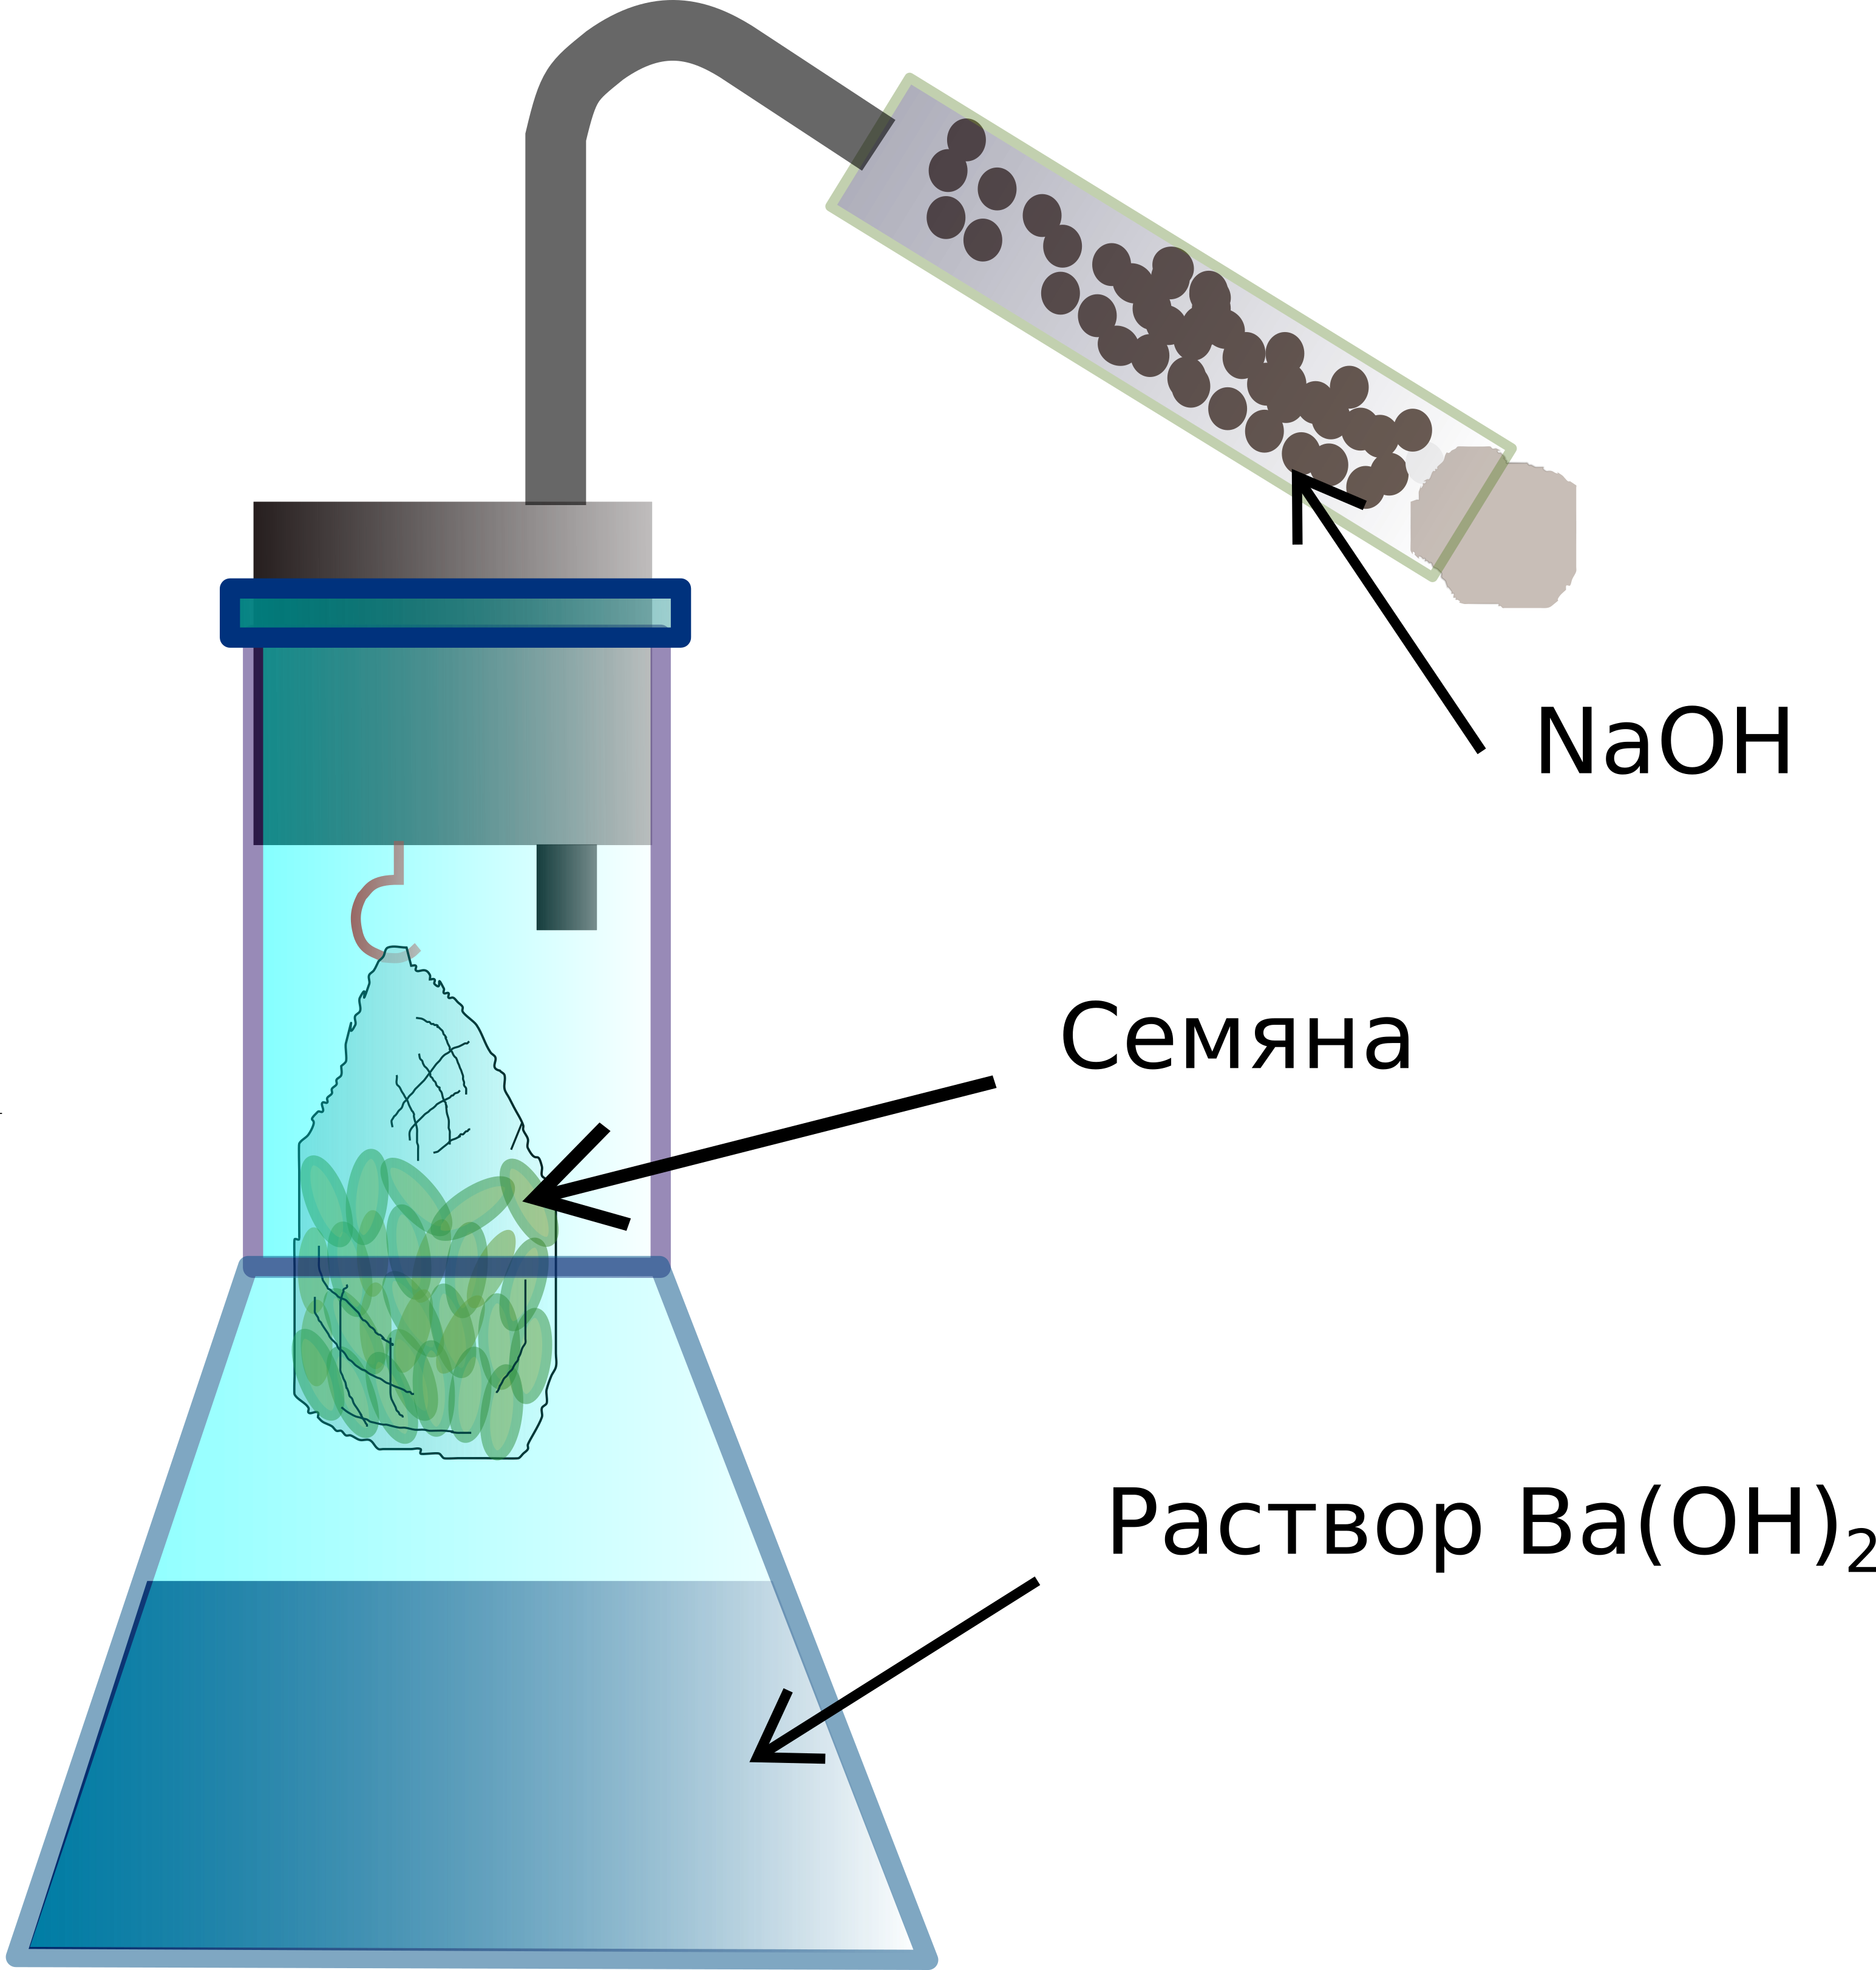
\includegraphics[width=0.5\linewidth]{pictures/breazing_colba}
\caption{Прибор для измерения интенсивности дыхания}
\label{breazing_colba}
\end{figure}
%%%%%%%%%%%%%%%%%%%%%%%%%%%%%%%%%%%%%%%%%%%%%%%%%%%%%%%%%%%%%%%%%%%%%%%%%%%%%%%%%%%%%%%%%%%%%%%%%%%%%%%%%%%

\paragraph*{}Оставьте обе колбы на 1 час при комнатной температуре, при этом содержимое колб периодически осторожно перемешивают, покачивая колбы. Это необходимо для того, чтобы разрушить плёнку углекислого бария, которая со временем образуется на поверхности баритной воды и препятствует поглощению.

\paragraph*{}Одновременно с первым опытом, проведите такой же опыт на семенах, выдержанных при температуре 30 градусов. 

\subsubsection{Определение интенсивности дыхания}

\paragraph*{}Через 1 час извлеките из колбы мешочек с семенами, а в саму колбу добавьте три капли фенолфталеина и оттитруйте барит 0,1 н до слабо-розового окрашивания, исчезающего от одной капли кислоты. Так же оттитруйте барит и в контрольной колбе. При проведении титрования колбы надо закрыть пробкой, через которую проходит кончик пипетки, присоединённой к бутылке с баритом\footnote{При титровании необходимо свести до минимума контакт баритной воды и воздуха так как баритная вода будет продолжать связывать углекислый газ воздуха во время титрования, что приведет к искажению результатов опыта}.

\paragraph*{}интенсивность дыхания семян рассчитывается по формуле \ref{baoh_titr}:

\begin{equation}
	\label{baoh_titr}
	J = \frac{(a-b)K.2,2}{n}
\end{equation}

\paragraph*{}Где \textit{a} и \textit{b} - количество 0,1 н щавелевой кислоты, которая была израсходована на титрование барита в контрольном и опытном вариантах, мл; \textit{K} - поправка к титру 0,1 н раствора щавелевой кислоты; 2,2 - количество $CO_2$ мг, соответствующее 1 мл 0,1 н раствора щавелевой кислоты; \textit{n} - масса сухих семян г 

\paragraph*{}Параллельно определите дыхание семян при 30 градусах. Результаты опыта запишите по форме.

\paragraph*{}\textbf{Сделайте вывод} о влиянии температуры на интенсивность дыхания.

\subsection*{Вопросы для самоконтроля}

	\begin{itemize}
		\item В чем заключается значение дыхания для живых организмов?
		\item Напишите балансовое уравнение дыхания;
		\item Какие факторы влияют на интенсивность дыхания?
		\item Для чего применяется метод титрования. В чем заключается его сущность? Какие типы титрования существуют?
		
	\end{itemize}
	
\section*{\lbtitle Определение дыхательного коэффициента прорастающих семян}
\addcontentsline{toc}{section}{Определение дыхательного коэффициента прорастающих семян}

%\subsection*{Теоретические положения}

%\paragraph{}\efbox[margin=10pt,backgroundcolor=yellow]{
%	\begin{minipage}{0.95 \textwidth}
%	Дыхательный коэффициент (ДК) – это отношение количества $CO_2$, выделившегося в процессе дыхания, к поглощенному за это время кислороду ($CO{_2}/O{_2}$).
%	\end{minipage}
%	}	

%\paragraph{}Дыхательный коэффициент служит характеристикой калорийности субстрата и зависит от вида дыхательного субстрата и степени его окисленности. 

%\paragraph*{}В качестве субстрата для дыхания могут использоваться жиры, белки, углеводы и органические кислоты. Чем больше окислен материал, тем меньше поглощается кислорода воздуха, а значит и меньше выделяется энергии. Если в процессе дыхания используется углеводы, то ДК равен единице. Это следует из балансового уравнения окисления глюкозы \ref{glucosa_reaction}:

%\begin{equation}
%\label{glucosa_reaction}
%	C{_6}H_{12}O{_6} + 6O{_2} \rightarrow 6H{_2}O + 6CO{_2}
%\end{equation}
 

%\paragraph*{}В данном уравнении отношение $6CO{_2}/6O{_2}$ равно 1. При окислении жирных кислот и белков ДК будет меньше единицы так как они насыщены кислородом в меньшей степени, и, следовательно, на их окисление идет больше $O2$. Так, в случае окисления масляной кислоты \ref{oil_acide_reaction}:

%\begin{equation}
%\label{oil_acide_reaction}
%	CH{_3}-CH{_2}-CH{_2}-COOH + 5O{_2} \rightarrow 4H{_2}O + 4CO{_2} 
%\end{equation}

%ДК = $4CO{_2}/5O{_2}$ = 0,8

%\paragraph*{}При использовании в качестве субстрата дыхания более окисленных органических кислот, ДК будет больше единицы: 

%$C{_4}H{_4}O{_5} + 2,5O{_2} \rightarrow 2H{_2}O + 4CO{_2}$, 

%ДК =  $4CO{_2}/2,5O{2}$ = 1,6. 

\begin{footnotesize}

\paragraph*{}\textbf{Цель работы}: Определить дыхательный коэффициент  прорастающих семян гороха;

\paragraph*{}\textbf{Оборудование}: Наклюнувшиеся семена гороха, пробирка с притертой пробкой, изогнутая под прямым углом стеклянная трубка, линейка, штатив
для пробирок, фильтровальная бумага, фарфоровые чашки, пинцеты, пипетки, часы;

\paragraph*{}\textbf{Реактивы}: 20-ный\% раствор КОН, окрашенная вода в
химическом стаканчике;

\end{footnotesize}

\subsection*{Ход работы}

\paragraph*{}Поместите в пробирку проклюнувшиеся семена гороха таким образом, чтобы пробирка была заполнена семенами примерно до половины. 

\paragraph*{}В изогнутую трубку поместите каплю окрашенной жидкости. Для этого опустите трубку в стакан с окрашенной жидкостью, после чего противоположный конец трубки закройте пальцем. Затем закройте пробирку с семенами пробкой с изогнутой трубкой.

\paragraph*{}Собранный и готовый к опыту прибор должен выглядеть следующим образом (рисунок \ref{breazing_index}). 

%%%%%%%%%%%%%%%%%%%%%%%%%%%%%%%%%%%%%%%%%%%%%%%%%%%%%%%%%%%%%%%%%%%%%%%%%%%%%%%%%%%%%%%%%%%%%%%%%%%%%%%%%%% 
\begin{figure}[h!]
  \centering
       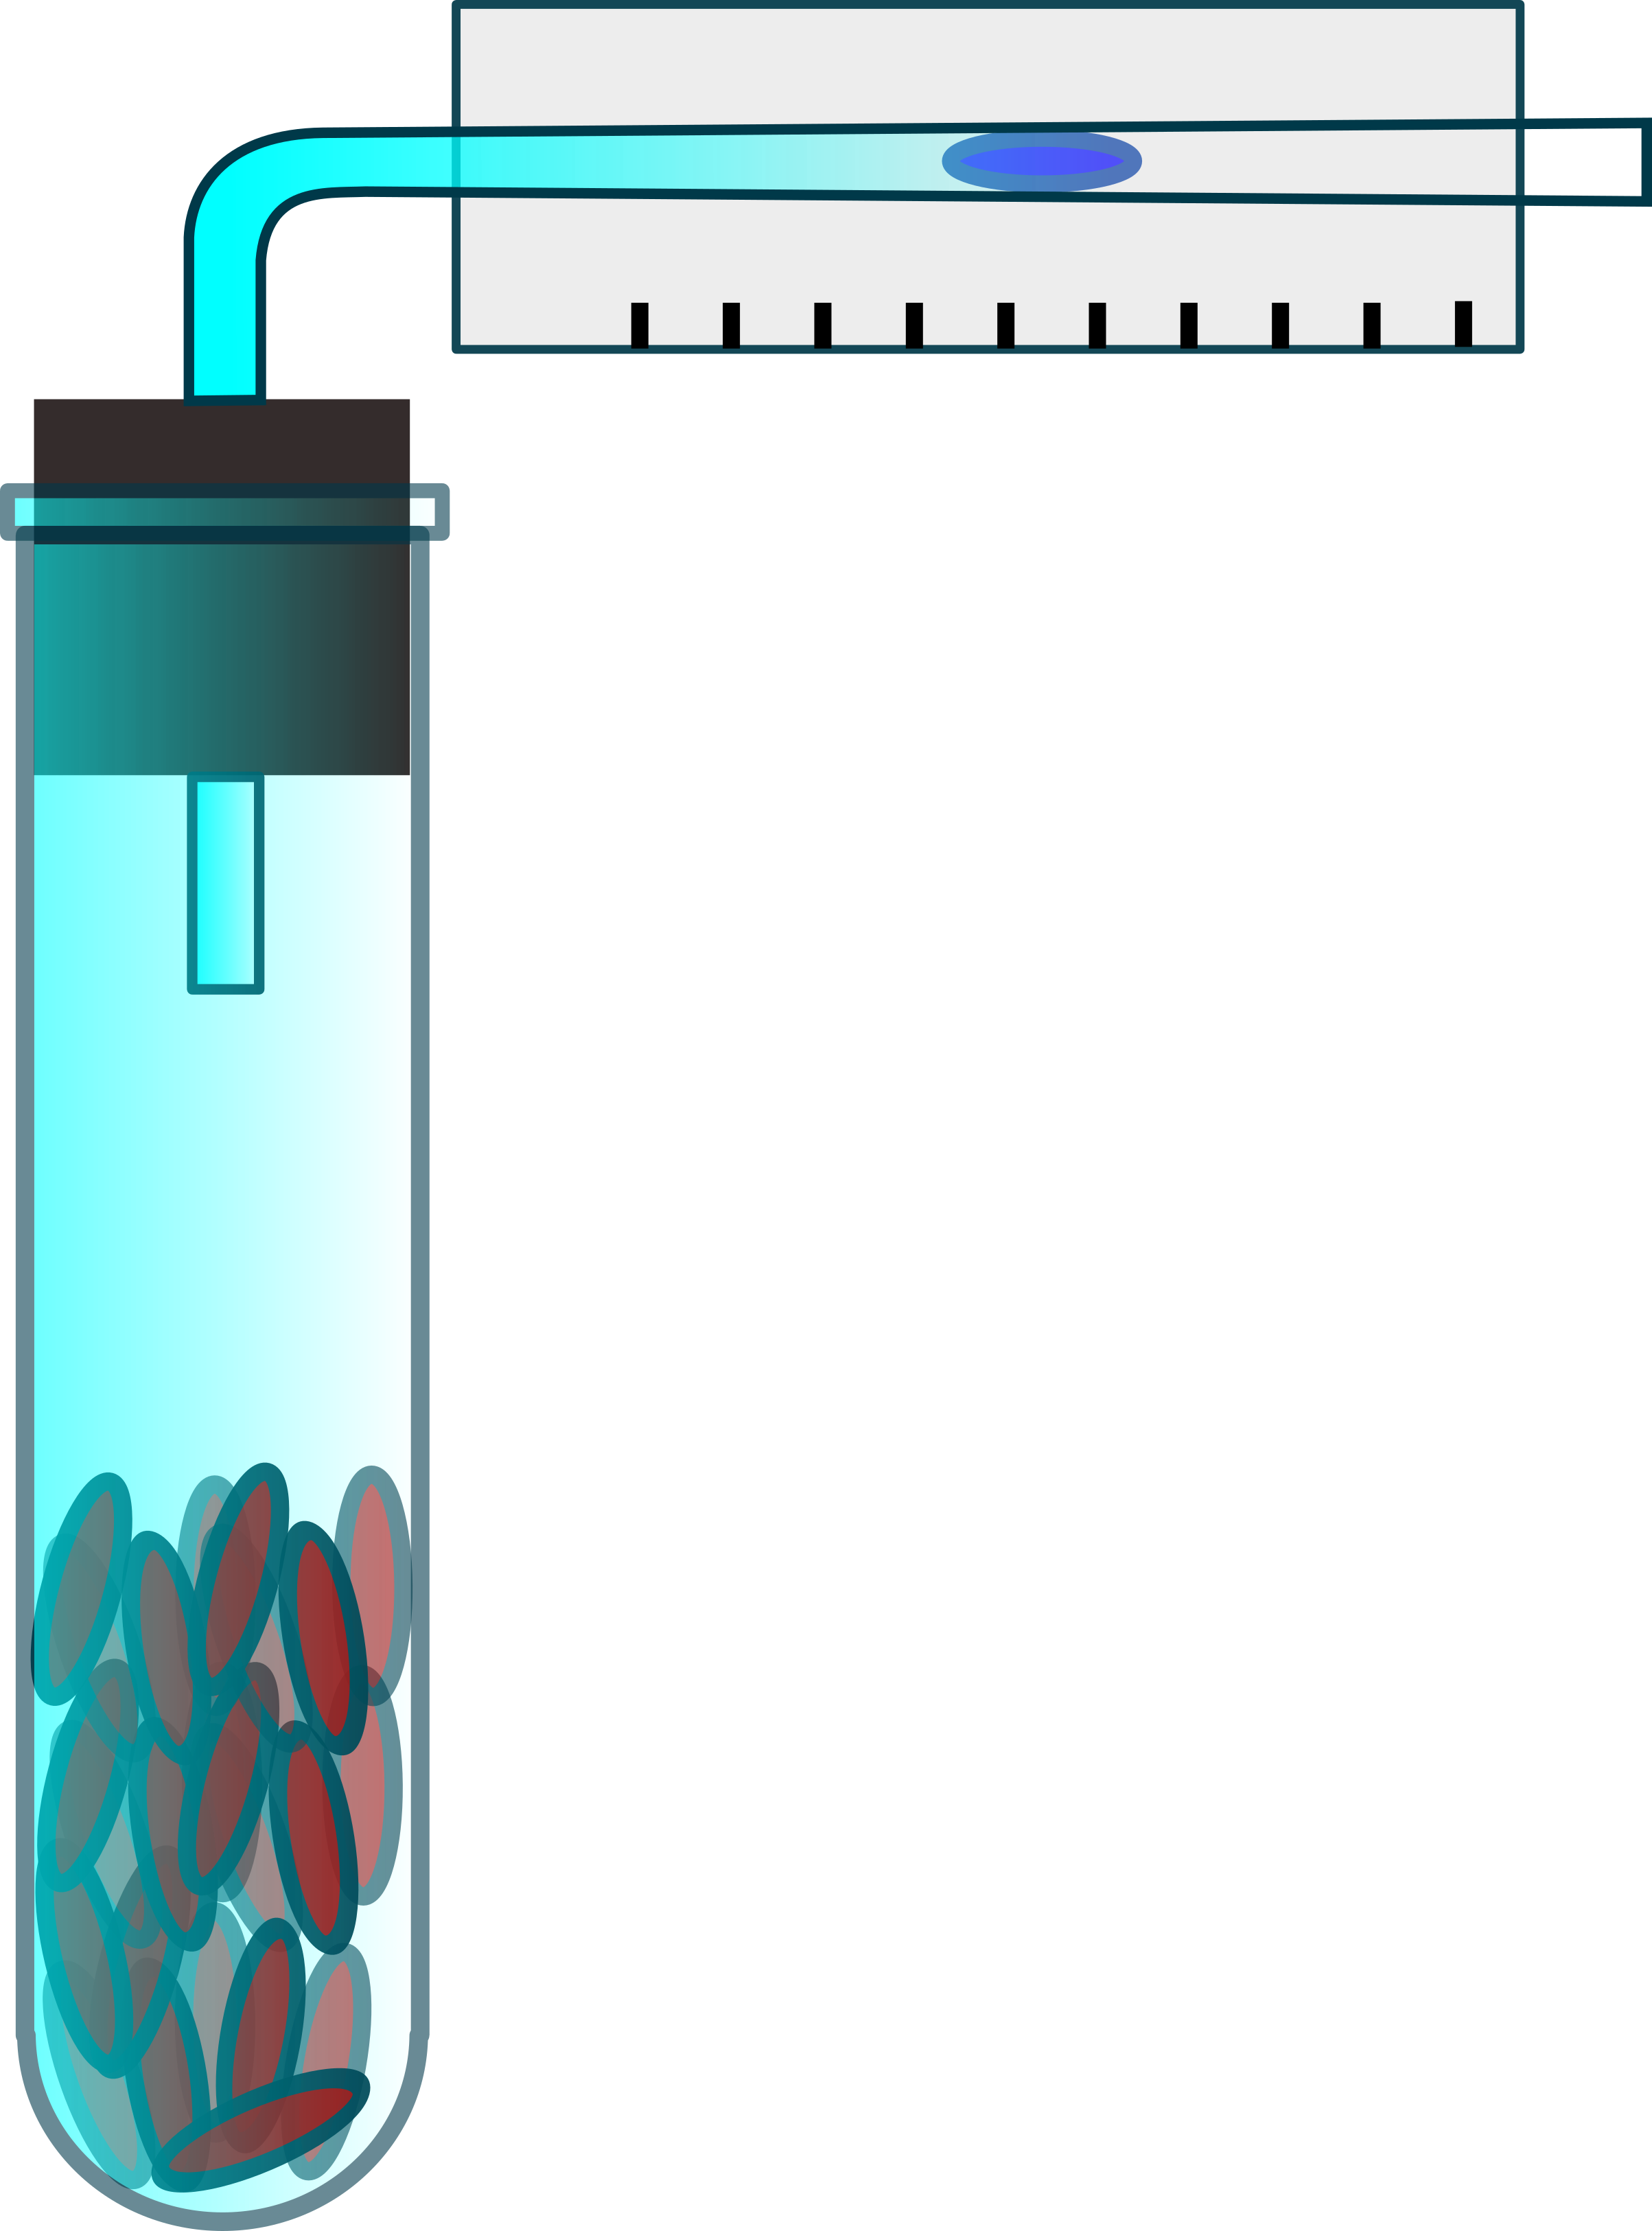
\includegraphics[width=0.3\linewidth]{pictures/breazing_index}
\caption{Прибор для измерения дыхательного коэффициента}
\label{breazing_index}
\end{figure}
%%%%%%%%%%%%%%%%%%%%%%%%%%%%%%%%%%%%%%%%%%%%%%%%%%%%%%%%%%%%%%%%%%%%%%%%%%%%%%%%%%%%%%%%%%%%%%%%%%%%%%%%%%%

\paragraph*{}Собранный таким образом прибор помещается в штатив. Положение мениска, образованного окрашенной жидкостью отмечается в начале опыта и затем через каждые 5 минут. Опыт продолжатся 15 минут.

\paragraph*{}На основании проделанных в результате опыта измерений, вычислите среднее расстояние, пройденное каплей за 5 минут (А). Это расстояние соответствует разности между объемами поглощенного кислорода и выделенного углекислого газа.

\paragraph*{}По окончании первой серии измерений, в пробирку с семенами пинцетом поместите фильтровальная бумага, смоченная раствором NaOH. Снова закройте пробирку пробкой с изогнутой трубкой. Отметет положение мениска в начале опыта и затем в течении 15 минут через каждые 5 минут. Расстояние, пройденное окрашенной каплей в трубке, будет соответствовать количеству поглощенного кислорода, так как выделившийся в ходе дыхания  углекислый газ будет поглощаться раствором NaOH.

\paragraph*{}Дыхательный коэффициент вычисляется по формуле \ref{k_breaz}:

\begin{equation}
  \label{k_breaz}
  k = \frac{CO{_2}}{O{_2}} = \frac{(B - A)}{B}
\end{equation} 

\paragraph*{}Где \textit{А} - количество выделившегося углекислого газа, измеренное во время первого опыта, \textit{B} - количество поглощенного кислорода, измеренное во время второго опыта.

\paragraph*{}Результаты наблюдения запишите в таблицу \ref{table_breezing_seeds}.

\begin{table}
\centering
	\label{table_breezing_seeds}
	\caption{Форма заполнения результатов}
	\begin{tabular}{|c|c|c|c|c|c|}
		\hline Условия & \multicolumn{4}{|c|}{Отсчет, мм 5 мин} & (В-А)/В \\ \cline{2-6}
		               &       1      &     2   &   3 & Среднее &         \\ 
		\hline Без щелочи (А)  &      &         &     &         &         \\
		\hline Со щелочью (Б)  &      &         &     &         &         \\
		\hline
	
	\end{tabular}
\end{table}

\paragraph*{}На основе измерения дыхательного коэффициента, \textbf{сделайте вывод} о природе субстрата, служащего для дыхания прорастающих семян.

\subsection*{Вопросы для самоконтроля}

\begin{itemize}
	\item Какие факторы будут влиять на интенсивность дыхания?
	\item При каких условиях случается выпревание озимых? Каким образом гибель растений от выпревания связанна с дыханием?
	\item В чем заключается роль кофермента НАД в процессе дыхания?
	\item В чем заключается сущность окислительного фосфорилирования?
	\item Какой процесс является общим как для брожения так и для аэробного дыхания? В чем сущность этого процесса?
	\item В чем заключается роль цикла Кребса для метаболизма растений?
\end{itemize}


%\chapter{Минеральное питание растения}

%\paragraph*{}Важнейшими \hypertarget{nutrition}{химическими} элементами, входящими в состав растения являются С, О, Н, N, Р, S. Среди этих элементов, углерод, кислород и водород поступают в организм растения из воздуха в виде воды и углекислого газ. В свою очередь Азот, фосфор, сера, а так же ряд других элементов, таких как калий, магний, железо, поступают из почвы через корневую систему в виде минеральных соединений.

%\paragraph*{}Все элементы в зависимости от их количественного содержания разделяются на макроэлементы (> 0,01\%) – N, Р, S, К, Са, Mg, Fe и микроэлементы (< 0,01\%) – Mn, Сu, Zn, В, Mo, О.

%\paragraph*{}Потребность растений в различных минеральных элементах может быть охарактеризована правилами, сформулированными  Ю. Либихом:

%\begin{itemize}
%	\item все элементы равнозначны и полное исключение любого из них приводит растение к гибели;
%	\item ни один из элементов не может быть заменён другим, даже близким по химическим свойствам, т. е. каждый элемент имеет своё специфическое физиологическое значение и по этой причине продуктивность культурных растений, в первую очередь, зависит от того питательного вещества (минерального элемента), который представлен в почве наиболее слабо. Данный закон получил название \textit{закона минимума Либиха}\cite{berezina_2009}. 
%\end{itemize}

%\paragraph*{}Таким образом, каждый из химических элементов, входящих в состав растения играет свою важную роль в метаболизме. Например такие элементы как C, O, H образуют структуру органических молекул, K, Na присутствуют в виде ионов участвуя в процессах регуляции метаболизма, Mn, Сu, Fe входят в состав активных центров ряда важных ферментов.

\section*{\lbtitle Рост корней пшеницы в чистой соли и смеси солей}
\addcontentsline{toc}{section}{Рост корней пшеницы в чистой соли и смеси солей}

%\subsection*{Теоретические положения}

%\paragraph*{}Корни растения поглощают из окружающей среды минеральные элементы в виде \hyperlink{ion}{ионов}. Часто ионы оказывают взаимное влияние на скорость поглощения, которое можно охарактеризовать как синергизм или антагонизм. Так ионы, имеющие одинаковый заряд, взаимно тормозят друг друга, и напротив ионы с противоположным зарядом ускоряют поступление друг дуга в растение.

%\paragraph{}\efbox[margin=10pt,backgroundcolor=yellow]{
%	\begin{minipage}{0.95 \textwidth}
%\paragraph*{}\textbf{Антагонизм} ионов это конкуренция между ионами одного заряда при поступлении в растение и как следствие уменьшение интенсивности их поглощения. Антагонистами являются ионы H$^+$, K$^+$, NH${_4}{^+}$, Ca$^{2+}$, Mg$^{2+}$, Cl$^-$, NO${_3}{^-}$, HCO${_3}{^-}$, SO${_4}{^2-}$, H$_2$PO${_4}{^-}$.

%\paragraph*{}\hyperlink{sinergism}{\textbf{Синергизм}} это явление, когда один ион способствует лучшему поглощению другого, например, Ca$^{2+}$ и K$^+$; Cl$^-$ и NO${_3}{^-}$.
%	\end{minipage}
%	}

%\paragraph*{}Подбирая различные концентрации отдельных ионов, можно составить такую их комбинацию, при которой данные растения будут развиваться лучше всего. Такой раствор называют \hyperlink{mixture}{уравновешенным} - то есть раствор нескольких солей, в котором не проявляется отрицательное действие на растение отдельных компонентов. 

\paragraph*{}\textbf{Цель работы}: Определить различия в характере роста пшеницы в растворе чистой соли и смеси солей.

\paragraph*{}\textbf{Оборудование}: Десятидневные проростки пшеницы. Конические колбы на 100 мл марля.

\paragraph*{}\textbf{Реактивы}: Растворы химически чистых солей - $KCl$, CaCl${_2}$, $NaCl$

	\subsection*{Ход работы}
	
\paragraph*{}Данная работа рассчитана на два занятия. В ходе первого из них ведётся закладка опыта, а в ходе второго — обработка полученных результатов.
	
	\subsubsection*{Первое занятие}
	
	\paragraph*{}Используя аналитические весы, сделайте навески и приготовьте растворы солей, согласно схемы опыта. Налейте приготовленные растворы в конические колбы объёмом 100 мл и закройте их горла марлевыми крышками. Высадите на каждую марлевую крышку одинаковое количество заранее приготовленных подростков пшеницы. Следите за тем, чтобы корни проростков были погружены в воду.
	
	\subsubsection*{Второе занятие}
	
	\paragraph*{}Спустя две недели измерьте высоту проростков, число и длину корней и сделайте соответствующие выводы о \hyperlink{growth_question}{влиянии} на рост корней чистой соли и смеси солей. Результат наблюдений запишите в таблицу. 
	
	\subsection*{Вопросы для самоконтроля}

	\begin{itemize}
		\item Какая частица называется \hypertarget{ion}{ионом}? Вспомните, какие ионы играют наиболее важную роль в жизни растений?
		\item \hypertarget{mixture}{Какой} раствор называется уравновешенным?
		\item Какую роль играют используемые в данном опыте минеральные элементы в жизни растений?
		\item Каковы механизмы поступления минеральных элементов в растение?
		\item В чем состоит суть явлений \hypertarget{sinergism}{синергизма и антогонизма} ионов?
		\item В каком растворе наблюдался наибольший рост \hypertarget{growth_question}{проростков}, а в каком рост проростков был сильнее всего угнетен? Почему? 
	\end{itemize}
	
\section*{\lbtitle Влияние отдельных элементов питательной смеси на рост растения}
\addcontentsline{toc}{section}{Влияние отдельных элементов питательной смеси на рост растения}

%\subsection*{Теоретические положения}

%\paragraph*{}Исключение из минерального питания растения хотя бы одного химического элемента приводит к нарушению обмена веществ растительного организма, проявляется в замедление роста растения и приводит к его последующей гибели. При этом наиболее быстро к видимым нарушениям обмена веществ приводит отсутствие таких элементов как азот и кальций. Роль наиболее важных элементов кратко описывается ниже:

%\begin{itemize}

%\item \hyperlink{nitrogen}{Азот} необходим для роста растений, так как входит в состав многих органических веществ, главным образом белков. 

%\item Калий увеличивает водоудерживающую способность протоплазмы клетки, и способствует поддержанию тургорного давления.

%\item \hyperlink{PS}{Сера} входит в состав аминокислот, являющихся мономерами белков. Соединения серы играют большую роль как регуляторы окислительно-восстановительного потенциала живой клетки.

%\item \hyperlink{PS}{Фосфор} входит в состав белков, нуклеиновых кислот, фосфатидов, ферментов, витаминов, фитина и других биологически активных веществ

%\item \hyperlink{MnMg}{Магний} входит в состав хлорофилла и, следовательно, необходим для фотосинтеза. 

%\item Кальций участвует в нейтрализации образующихся в тканях в процессе обмена веществ органических кислот, в частности щавелевой кислоты.

%\end{itemize}

%\paragraph*{}Кроме кальция нереутилизируемым являются многие минеральные элементы.

\begin{footnotesize}

\paragraph*{}\textbf{Цель работы}: Определить влияние недостатка отдельных минеральных элементов на рост и развитие растений;

\paragraph*{}\textbf{Оборудование}: Стеклянные банки емкостью 1 литр, бумага, деревянные пробки, бюретки на 50 мл, проростки растений;

\paragraph*{}\textbf{Реактивы}: Растворы химически чистых солей - KNO${_3}$, Ca(NO${_3}$)${_2}$, NaCl, KH${_2}$PO${_4}$, NaH${_2}$PO${_4}$, MgSO${_4}$ \textperiodcentered 7H${_2}$O, CaSO${_4}$ \textperiodcentered 2H${_2}O$, MnSO${_4}$, 0,5\% раствор цитрата железа, раствор борной кислоты;

\end{footnotesize}


\subsection*{Ход работы}	
	
\subsubsection*{Приготовление питательной среды}
	
\paragraph*{}Приготовьте для опыта полную питательную смесь по Хогланду-Снайдерсу, а так же смеси из состава которых исключены по отдельности азот, фосфор и калий. Следует учесть, что при исключении из смеси отдельного элемента питания, связанные с ним элементы необходимо внести в эквивалентных количествах, в виде солей, не содержащих исключаемый элемент \footnote{Это делается для чистоты эксперимента, чтобы исключить влияние на растение  связанных элементов. Например удаляя калий в форме   K{H$_2$}PO{$_4$} вместе с ним мы удаляем еще и фосфор входящий в состав иона {H$_2$}PO{$_4^-$}}. 

\paragraph*{}Перед приготовлением питательного раствора составьте рабочую таблицу, где укажите необходимое количество солей на выбранный объем (таблица \ref{hogland_mixture}).

\label{hogland_mixture}	
%\begin{longtable}{|p{0.2\linewidth}|p{0.2\linewidth}|p{0.15\linewidth}|p{0.15\linewidth}|p{0.15\linewidth}|}
\begin{longtable}{|c|c|c|c|c|}
\caption{Рабочая таблица для приготовления питательной смеси}\\
\hline  \multirow{1}{*}{Соль} & \multirow{1}{*}{Масса соли для маточного раствора} & \multicolumn{3}{c|}{Количество маточного раствора} \\ \cline{3-5}                                                                                         
	          
  & & 1 норма                & 0.5 нормы	        & 0.2 нормы	\\

\hline \multicolumn{5}{|c|}{Микроэлементы на 10 л раствора} \\

\hline KNO$_3$ & 510 & 10.0 & 5.0 & 2.0 \\                                                                                  
\hline Ca(NO${_3}$)${_2}$ & 10 \% раствор & 8.2 & 4.1 & 1.6 \\                                                                                  
\hline K{H$_2$}PO{$_4$} & 136 & 10.0 & 5.0 & 2.0 \\                                                                                  
\hline MgSO${_4}$ \textperiodcentered 7H${_2}$O & 490 & 10.0 & 5.0 & 2.0 \\                                                                                  

\hline \multicolumn{5}{|c|}{Микроэлементы на 2 л раствора} \\

\hline MnCl$_{2}$ \textperiodcentered 4H${_2}$O & 0.35 &  &  &  \\                                                                                  
\hline H$_{3}$BO$_{3}$ & 0.55 &  &  &  \\                                                                                  
\hline ZnSO${_4}$ & 0.05 &  &  &  \\
\hline CuSO${_4}$ & 0.05 &  &  &  \\                                                                                  
\hline MoO${_2}$ & 0.024 &  &  &  \\
\hline FeSO${_4}$ \textperiodcentered 7H${_2}$O & 4.0 &  &  &  \\
\hline

\end{longtable}

\paragraph*{\warningsign}Во избежании размножения водорослей, приготовленный раствор нужно хранить в посуде из темного стекла.
	
\subsubsection*{Смесь без азота}
	
\paragraph*{}В питательный раствор азот входит в виде нитратов Ca(NO${_3}$)${_2}$ и KNO$_3$. Для того чтобы сохранить концентрацию ионов K+ и Ca2+ в данном растворе, нитраты калия и кальция заменяются на KCl и CaSO${_4}$ \textperiodcentered 2H${_2}O$ соответственно.
	
	\paragraph*{Расчет массы \hypertarget{potashyum_mass}{KCl}} которую нужно внести в питательную смесь вместо KNO$_3$, производится исходя из того что 1 моль KNO$_3$\footnote{молярная масса KNO$_3$ составляет 101 г/моль.} содержит 40 г калия. Массу калия, содержащегося в 510 мг KNO$_3$ можно  рассчитать по пропорции
	
	\begin{equation}
		\frac{110 g_{KNO_3} - 40 g_{K}}{0,51 g_{KNO_3} - x g_{K}}
	\end{equation}	 

\paragraph*{}Отсюда	

\begin{equation}
		x = \frac{40 * 0,51}{110} = 0,19
	\end{equation}
	
\paragraph*{}Определив количество калия, содержащиеся в 510 мг KNO$_3$ можно определить, какое количество KCl необходимо для того чтобы в растворе содержалось 0,19 г калия. Масса KCl так же рассчитывается по пропорции:

	\begin{equation}
		\frac{75 g_{KCl} - 39 g_{K}}{x g_{KCl} - 0,19 g_{K}}
	\end{equation}
	
\paragraph*{}Отсюда:

\begin{equation}
		x = \frac{75*0,19}{39} = 0,37
	\end{equation}
	
\paragraph*{}Таким образом, для  того чтобы сохранить в питательной смеси нужное количество калия, вместо 0,51 г KNO$_3$ в смесь необходимо внести 0,37 г KCl

\paragraph*{Расчет массы KCl и CaSO${_4}$ \textperiodcentered 2H${_2}O$} которую необходимо внести вместо Ca(NO${_3}$)${_2}$ проводят по аналогичной схеме.

\subsubsection*{Смесь без фосфора}

\paragraph*{}Фосфор в питательной смеси содержится в виде гидрофосфта калия - KH${_2}$PO${_4}$. При исключении из смеси фосфора данная соль заменяется на KCl.

\paragraph*{Расчет массы KH${_2}$PO${_4}$} производят аналогично расчетам массы \hyperlink{potashyum_mass}{калия}.

\begin{equation}
	\frac{KH{_2}PO{_4} - K}{136 - 39}
\end{equation}

\begin{equation}
		x = \frac{39*0,136}{136} = 0,04
	\end{equation}

\begin{equation}
	\frac{KCl - K}{75 - 39}
\end{equation}

\begin{equation}
		x = \frac{74*0,04}{39} = 0,08
	\end{equation}
	
\paragraph*{}Таким образом, вместо 0,136 г KH${_2}$PO${_4}$ необходимо взять 0,08  KCl.

\subsubsection*{Смесь без калия}

\paragraph*{}Вместо гидрофосфата калия KH${_2}$PO${_4}$ в питательную смесь необходимо внести гидрофосфат натрия NaH${_2}$PO${_4}$ а вместо нитрата калия KNO${_3}$ - нитрата натрия - NaNO${_3}$.

\paragraph*{}Расчет массы данных веществ производится описанным \hyperlink{potashyum_mass}{выше} способом:

\begin{equation}
	\frac{KH{_2}PO{_4} - P}{136 - 31}
\end{equation}

\begin{equation}
		x = \frac{31*0,136}{136} = 0,031
	\end{equation}
	
\begin{equation}
	\frac{NaH{_2}PO{_4} - P}{138 - 31}
\end{equation}
	
\begin{equation}
		x = \frac{138*0,031}{31} = 0,138
	\end{equation}

\paragraph{}Следовательно, на 1 л смеси необходимо взять 0,138 г гидрофосфата натрия. Аналогичным образом рассчитывают массу NaNO${_3}$ необходимую для замены в смеси нитрата калия KNO${_3}$.

	\subsection*{Вопросы для самоконтроля}
	
	\begin{itemize}
		
		\item Какие элементы относятся к макро-, а какие к микроэлементам?
		\item Какие элементы являются реутилизируемыми а какие не реутилизируемыми? 
		\item По каким признакам можно отличить нехватку у растения рутилизированных элементов от нехватки нереутилизируемых?
		\item В чем заключается роль \hypertarget{nitrogen}{азота} в обмене веществ растения? Каковы признаки нехватки данного элемента для растения?
		\item В чем заключается роль в обмене веществ растительного организма \hypertarget{PS}{фосфора и серы}? Каковы признаки нехватки данных элементов для растения?
		\item В чем заключается роль в обмене веществ растительного организма \hypertarget{MnMg}{марганца и магния}? Каковы признаки нехватки данных элементов для растения?
	\end{itemize}
	

%\chapter{Рост и развитие растения}

%\paragraph*{}
%\efbox[margin=10pt,backgroundcolor=yellow]{
%	\begin{minipage}{0.95 \textwidth}
%		\textbf{\hypertarget{growth}{Рост}} – необратимое увеличение размеров и массы клетки, органа или всего организма, обусловленное новообразованием элементов их структур.
%	\end{minipage}
%	}

%\paragraph*{}Рост растения осуществляется при участии специализированных образовательных тканей - меристем. Различают апикальные меристемы, расположенные на \hyperlink{where_meristems_plased}{кончиках корня} и стебля и обеспечивающие рост стебля в высоту, латеральные меристемы, обеспечивающие утолщение стебля и корня и вставочные меристемы, расположенные в междоузлиях и так же отвечающие за рост растения в высоту.

%\paragraph*{}Процессы роста растения регулируются при участии различных \hyperlink{chem_regulators}{химических веществ} оказывающих гормоноподобное действие. Среди регуляторов роста наиболее важными являются ауксины, гиббереллины и цитокины. 

%\paragraph*{}Ауксины создаются в верхушках (апексах) стеблей и корней, затем они перемещаются в зону растяжения клеток — и способствуют их удлинению. Ауксины влияют на рост колеоптилей злаков, стеблей, листьев и корней растений, вызывают изгибы органов, задерживают опадение листьев и завязей, а также способствуют образованию корней у черенков. Наиболее распространенным ауксином является $\beta$-индолил-3-уксусная кислота (ИУК). Ауксин передвигается только вниз по стеблю.

%\paragraph*{}Гиббереллины значительно сильнее усиливают рост стебля, чем ауксины. Рост происходит в результате удлинения стебля, а не образования новых междоузлий. Без гиббереллинов растения получаются карликовыми. Характерная особенность гиббереллинов — проявлять свои свойства только в целом растении, а не в изолированных его частях.

%\paragraph*{}Кинины, или цитокинины, стимулируют клеточное деление. 

%\paragraph*{}Регуляторы роста могут так же влиять на \hyperlink{chem_ontogenesis}{этапы развития} (онтогенеза) растительного организма. Так ауксины задерживают опадение листьев и завязей, а также способствуют образованию корней у черенков, а цитокины активировать прорастание семян и дифференциацию почек.

%\paragraph*{}\efbox[margin=10pt,backgroundcolor=yellow]{
%	\begin{minipage}{0.95 \textwidth}Развитие – это качественные изменения в структуре и функциональной активности растения и его частей в процессе онтогенеза. 
%	\end{minipage}
%	}

%\paragraph*{}В онтогенезе каждого растения выделяют такие этапы, как эмбриональный - который длится от оплодотворения до прорастания семени, ювенильный - от прорастания до первого цветения, этап зрелости который длится все время пока растение способно плодоносить и этап старости и смерти.

%\paragraph*{}В зависимости от особенностей жизненного цикла, все растения разделяют на \textit{монокарпические} (плодоносящие один раз) и \textit{поликарпические} (плодоносящие многократно). К монокарпическим относятся: все однолетние растения, некоторые двулетние и многолетние. Большинство многолетних растений поликарпические.


\section*{\lbtitle Определение зон роста в органах растения}
\addcontentsline{toc}{section}{Определение зон роста в органах растения}

%\subsection*{Теоретические положения}

%\paragraph*{}Рост стебля в высоту, как было сказано выше происходит за счет клеток меристем: апикальной — на кончике стебля и интеркаллярных, расположенных в узлах стебля. Именно в местах расположения меристем наблюдается наиболее интенсивных рост стебля. Таким образом величина прироста стебля по всей длине будет неодинаковой.Таким образом величина прироста стебля по всей длине будет неодинаковой.

\paragraph*{}\textbf{Цель работы}: Определить расположение зон наиболее интенсивного роста побега

\paragraph*{}\textbf{Оборудование}: Проростки гороха с корнями длинной 1,5-2 см, проростки подсолнечника, чёрная туш и перо или черный маркер, древесные опилки, препаровальные иглы, миллиметровая бумага.

\subsection*{Ход работы}

\paragraph*{}Данная работа рассчитана на два занятия. В ходе первого из них ведётся закладка опыта, а в ходе второго — обработка полученных результатов.

	\subsubsection*{Первое занятие}
	
	\paragraph*{}Прорастите во влажных опилках семена гороха (5 штук). Для обеспечения строго вертикального роста корней, в опилках стеклянной палочкой проделайте вертикальные углубления глубиной в несколько сантиметров. 
	
	\paragraph*{}На предварительно подсушенный фильтровальной бумагой корень гороха нанесите метки, расстояние между которыми составляет 3 мм. Метки должны быть тонкими и хорошо заметными. 
	
	\paragraph*{}\warningsign С помощью туши и пера метки получаются более тонкими, а измерения более точными. Однако при нанесении меток тушью соблюдайте осторожность так как можете случайно поранить пером стебель или корень проростка.
	
	\paragraph*{}Для определения зон роста побега, нанесите метки на расстоянии 3 мм на побег проростка подсолнечника. Всего 10 меток, начиная от верхушки. Затем поместите проростки с нанесёнными метками тёмное место\footnote{В условиях недостатка света побег начнет интенсивно расти, вытягиваться и, вследствие этого рост будет выражен более отчетливо.}.
	
	\subsubsection*{Второе занятие}
	
	\paragraph*{}Измерьте расстояние между метками на корнях гороха и побегах подсолнечника, на основание данных измерения нескольких растений вычислите среднесуточный прирост корня и стебля на разных участках. Запишите результаты опыта в \ref{growth_form}.
	
	\paragraph*{}По результатам измерения постройте график роста корня, где по оси абсцисс откладывается номер отрезка, а по оси ординат - прирост (рисунок \ref{growth_graf}). 
	
\begin{table}[h!]
\centering
\label{growth_form}
\caption{Форма записи результатов}
\begin{tabular}{|c|c|c|c|c|c|c|c|c|c|c|c|c|c|c|c|}
\hline & \multicolumn{15}{|c|}{Зона прироста мм}  \\ \cline{2-16}
 Номер проростка & 1 & 2 & 3 & 4 & 5 & 6 & 7 & 8 & 9 & 10 & 11 & 12 & 13 & 14 & 15 \\
\hline 1 & & & & & & & & & & & & & & & \\
\hline 2 & & & & & & & & & & & & & & & \\
\hline 3 & & & & & & & & & & & & & & & \\
\hline 4 & & & & & & & & & & & & & & & \\
\hline 5 & & & & & & & & & & & & & & & \\
\hline


\end{tabular}

\end{table}

\begin{figure}[h!]
\centering
\label{growth_graf}
\caption{Форма для построения графика}
\begin{tikzpicture}
	%Raster zeichnen
	\draw [color=gray!50]  [step=5mm] (0,0) grid (14,7);
	% Achsen zeichnen
	\draw[->,thick] (0,0) -- (15,0) node[right] {$x$};
	\draw[->,thick] (0,0) -- (0,8) node[above] {$y$};
	% Achsen beschriften
	\draw (1,-.2) -- (1,0) node[below=4pt] {$\scriptstyle 1$};
	\draw (2,-.2) -- (2,0) node[below=4pt] {$\scriptstyle 2$};
	\draw (3,-.2) -- (3,0) node[below=4pt] {$\scriptstyle 3$};
	\draw (4,-.2) -- (4,0) node[below=4pt] {$\scriptstyle 4$};
	\draw (5,-.2) -- (5,0) node[below=4pt] {$\scriptstyle 5$};
	\draw (6,-.2) -- (6,0) node[below=4pt] {$\scriptstyle 6$};
	\draw (7,-.2) -- (7,0) node[below=4pt] {$\scriptstyle 7$};	
	\draw (8,-.2) -- (8,0) node[below=4pt] {$\scriptstyle 8$};
	\draw (9,-.2) -- (9,0) node[below=4pt] {$\scriptstyle 9$};
	\draw (10,-.2) -- (10,0) node[below=4pt] {$\scriptstyle 10$};
	\draw (11,-.2) -- (11,0) node[below=4pt] {$\scriptstyle 11$};
	\draw (12,-.2) -- (12,0) node[below=4pt] {$\scriptstyle 12$};
	\draw (13,-.2) -- (13,0) node[below=4pt] {$\scriptstyle 13$};
	\draw (14,-.2) -- (14,0) node[below=4pt] {$\scriptstyle 14$};
	\foreach \y in {0,0,0,1,2,3,4,5,6,7}
	\draw (-.1,\y) -- (.1,\y) node[left=4pt] {$\scriptstyle\y$};
	\node[label={[label distance=-4.0cm,text depth=-1ex,rotate=90]left:Прирост (мм)}] at (-1,.10) {};
	\node[label={[label distance=6cm,text depth=-8ex]right:Номер отрезка}] at (0,-0.1) {};
\end{tikzpicture}
\end{figure}
	
\paragraph*{}На основании наблюдений, \textbf{сделайте вывод} о том, где расположены зоны наиболее интенсивного роста растения. С расположением каких образовательных тканей они связаны.

	\subsection*{Вопросы для самоконтроля}

	\begin{itemize}
		\item \hypertarget{where_meristems_plased}{Где} расположены основные образовательные ткани растения?
		\item Какие \hypertarget{chem_regulators}{гормоны} регулируют рост растения, в чем особенности регуляции роста этими гормонами?
		\item Как растительные гормоны влияют на этапы \hypertarget{chem_ontogenesis}{онтогенеза} растительного организма?
		\item Что такое тропизмы? Какие основные тропизмы проявляет организм растения?
		\item Что такое клеточный цикл? Какие события происходят на каждом из этапов клеточного цикла?
		\item На каком из этапов онтогенез растительная клетка способна к делению?
	\end{itemize}

\section*{\lbtitle Выявление апикального доминирования у гороха}
\addcontentsline{toc}{section}{Выявление апикального доминирования у гороха}

%\subsection*{Теоретические положения}

%\paragraph*{}Как известно, у многих растений верхушка подавляет развитие боковых побегов и пробуждение спящих почек \cite{fzr_ermakov}. Это явление получило название апикальное доминирование. Удаление или повреждение верхушечной почки снимает апикальное доминирование, в следствии чего спящие почки пробуждаются а рост боковых побегов усиливается.

%\paragraph*{}Горох это растение, у которого апикальное доминирование выражено довольно сильно. Это можно обнаружить, если удалить верхушку главного побега. Рост боковых побегов начинается уже через несколько дней после удаления верхушки.

\paragraph*{}\textbf{Цель работы}: Выявить явление апикального доминирования на примере растений гороха.
\paragraph*{}\textbf{Оборудование}: Сосуды с молодыми растениями гороха, бритвы, линейки.

\subsection*{Ход работы}

	\subsubsection*{Первое занятие}
	
	\paragraph*{}Среди имеющихся молодых растений, срежьте у двух  лезвием верхушку, а одно растение оставьте нетронутым в качестве контроля. Сосуды с растениями необходимо поместить в теплицу или климатостат.
	
	\subsubsection*{Второе занятие}
	
	\paragraph*{}На следующие занятие сравните высоту побега, количество и размер боковых побегов у интактных (не поврежденных) и декапилированных (лишенных верхушки) растений гороха. Результаты сравнения занесите в отчет в виде таблицы.
	
\subsection*{Вопросы для самоконтроля}

\begin{itemize}
	\item Чем рост отличается от развития?
	\item Какие растительные гормоны-стимуляторы роста вы знаете? Какие из них стимулируют рост путем растяжения клеток, а какие путем деления клеток?
	\item Какие растительные ткани отвечают за рост растения? В чем заключаются гистологические особенности строения этих тканей?
	\item Опираясь на результаты данной лабораторной работы, опишите, в чем заключается смысл такого агротехнического приема как пикировка?
	\item Перечислите и охарактеризуйте этапы развития растительного организма.
\end{itemize}
	
%\chapter{Приспособление и устойчивость растений}

%\paragraph*{}\efbox[margin=10pt,backgroundcolor=yellow]{
%	\begin{minipage}{0.95 \textwidth}Стресс это общая неспецифическая адаптационная реакция организма на действие любых неблагоприятных факторов, которые носят название стрессоры.
%	\end{minipage}
%	}

%\paragraph*{}В процессе развития стрессовой реакции растительный организм проходит  три стадии: 
%\begin{itemize}
%	\item первичная стрессовая реакция,
%	\item адаптация,
%	\item истощение.
%\end{itemize}

%\paragraph*{}Устойчивость растений к стрессору зависит и от фазы онтогенеза. Так, наиболее устойчивы растения, находящиеся в состоянии покоя а наиболее чувствительны растения в молодом возрасте.
 
%\paragraph*{}Ответ на стрессовое воздействие прослеживается на разных уровнях организации. так на уровне клетки наблюдается  

%\begin{itemize}
%	\item Повышение проницаемости мембран, деполяризация мембранного потенциала плазмалеммы.
%	\item Сдвиг рН цитоплазмы в кислую сторону.
%	\item Усиление поглощения кислорода, ускоренная трата АТФ, развитие свободнорадикальных процессов.
%	\item	Активация синтеза стрессовых белков.
%\end{itemize}

%\paragraph*{}Эти реакции направлены на защиту внутриклеточных структур и устранение неблагоприятных изменений в клетках. В невысоких дозах повторяющиеся стрессы приводят к закаливанию организма. Закаливание к одному стрессору способствует повышению устойчивости организма и другим повреждающим факторам.

\section*{\lbtitle Выявление защитного действия сахаров на протоплазму}
\addcontentsline{toc}{section}{Выявление защитного действия сахаров на протоплазму}

%\subsection*{Теоретические положения}

%\paragraph*{}Под воздействием отрицательных температур в межклетниках образуются кристаллы льда, которые оттягивают на себя воду из близлежащих клеток. Таким образом клетки подвергаются обезвоживанию, при определенной степени которого происходит коагуляция белков цитоплазмы. Кроме того, кристаллы льда могут образовываться и внутри клеток, нанося им тем самым механические повреждения.


%\paragraph*{}Увеличение в цитоплазме клеток концентрации растворимых сахаров увеличивает водоудерживающую способность цитоплазмы клеток.

\begin{footnotesize}

\paragraph*{}\textbf{Цель работы}: Наблюдение защитного действия сахаров на цитоплазму;
\paragraph*{}\textbf{Оборудование}: Корнеплод свеклы, термометры, скальпели, бритвенные лезвия, пробирки, микроскопы, предметные стекла, карандаш по стеклу, фильтровальная бумага;

\paragraph*{}\textbf{Реактивы}: раствор сахарозы концентрацией 0,1 и 0,5 M, NaCl, лед;

\end{footnotesize}

\subsection*{Ход работы}

\paragraph*{}Из корнеплода свёклы лезвием вырежьте высечки размером 5x5x5 см, которые затем промывают водой. Приготовленные таким образом высечки поместите в три пробирки по 3 высечки в каждую.

\paragraph*{}Первую пробирку наполните водой, вторую – 0,1 м, а третью - 0,5 м раствором сахарозы. Предварительно подписанные пробирки поместите на 20 минут в охладительную смесь, состоящую из трёх частей льда и одной части NaCl.

\paragraph*{}По прошествии 20-минут разморозьте пробирки и отметьте, как изменилась окраска жидкости в пробирках. Затем извлеките высечки из пробирок и с помощью острого лезвия изготовьте из них тонкие срезы, которые поместите на предметное стекло в капле того же растворе, в котором они находились. Подсчитайте количество обесцветившихся клеток в поле зрения микроскопа. Результат запишите в таблицу \ref{plasmolis_table}.

\begin{table}[h!]
\centering
\label{plasmolis_table}
	\begin{tabular}{|c|c|c|c|c|}
	
		\hline Условия &	\multicolumn{2}{c|}{Число клеток в поле зрения} & Окрашенные/Неокрашенные клетки & Вывод \\ \cline{2-5}
		 & Окрашеные & Неокрашеные & & \\
		\hline Вода & & & & \\
		\hline Сахароза 0,5 моль & & & & \\
		\hline Сахароза 0,1 моль & & & & \\
		\hline
	
	\end{tabular}
\end{table}

\subsection*{Вопросы для самоконтроля}

